% !TeX spellcheck = sl_SI
% vim: set spell spelllang=sl:
% za preverjanje črkovanja, če se uporablja Texstudio ali vim
\documentclass[12pt,a4paper,twoside]{article}
\usepackage[utf8]{inputenc}  % pravilno razpoznavanje unicode znakov

% NASLEDNJE UKAZE USTREZNO POPRAVI
\newcommand{\program}{Pedagoška matematika} % ime studijskega programa
\newcommand{\imeavtorja}{Simon Besednjak} % ime avtorja
\newcommand{\imementorja}{prof.~dr.~Marjetka Knez} % akademski naziv in ime mentorja, uporabi poln naziv, prof.~dr.~, doc.~dr., ali izr.~prof.~dr.
\newcommand{\imesomentorja}{} % akademski naziv in ime somentorja, če ga imate
\newcommand{\naslovdela}{Dvojne PH krivulje}
\newcommand{\letnica}{2021} % letnica magistriranja
\newcommand{\opis}{Delo obravnava lastnosti krivulj z pitagorejskih hodografom.}  % Opis dela v eni povedi. Ne sme vsebovati matematičnih simbolov v $ $.
\newcommand{\kljucnebesede}{PH krivulje\sep dvojne PH krivulje} % ključne besede, ločene z \sep, da se PDF metapodatki prav procesirajo
\newcommand{\keywords}{PH curves\sep double PH curves} % ključne besede v angleščini
\newcommand{\organization}{Univerza v Ljubljani, Fakulteta za matematiko in fiziko} % fakulteta
\newcommand{\literatura}{literatura}  % pot do datoteke z literaturo (brez .bib končnice)
\newcommand{\sep}{, }  % separator med ključnimi besedami v besedilu
% KONEC PODATKOV

\usepackage{bibentry}         % za navajanje literature v programu dela s celim imenom
\nobibliography{\literatura}
\newcommand{\plancite}[1]{\item[\cite{#1}] \bibentry{#1}} % citiranje v programu dela

\usepackage{filecontents}  % za pisanje datoteke s PDF metapodatki
\usepackage{silence} \WarningFilter{latex}{Overwriting file}  % odstrani annoying warning o obstoju datoteke
% datoteka s PDF metapodatki, zgenerira se kot magisterij.xmpdata
\begin{filecontents*}{\jobname.xmpdata}
  \Title{\naslovdela}
  \Author{\imeavtorja}
  \Keywords{\kljucnebesede}
  \Subject{matematika}
  \Org{\organization}
\end{filecontents*}

\usepackage[a-1b]{pdfx}  % zgenerira PDF v tem PDF/A-1b formatu, kot zahteva knjižnica
\hypersetup{bookmarksopen, bookmarksdepth=3, colorlinks=true,
  linkcolor=black, anchorcolor=black, citecolor=black, filecolor=black,
  menucolor=black, runcolor=black, urlcolor=black, pdfencoding=auto,
  breaklinks=true, psdextra}

\usepackage[slovene]{babel}  % slovenščina
\usepackage[T1]{fontenc}     % naprednejše kodiranje fonta
\usepackage{amsmath,amssymb,amsfonts,amsthm} % matematični paketi
\usepackage{graphicx}     % za slike
\usepackage{emptypage}    % prazne strani so neoštevilčene, ampak so štete
\usepackage{units}        % fizikalne enote kot \unit[12]{kg} s polovico nedeljivega presledka, glej primer v kodi
\usepackage{makeidx}      % za stvarno kazalo, lahko zakomentiraš, če ne rabiš
\makeindex                % za stvarno kazalo, lahko zakomentiraš, če ne rabiš
% oblika strani
\usepackage[
  top=3cm,
  bottom=3cm,
  inner=3.5cm,      % margini za dvostransko tiskanje
  outer=2.5cm,
  footskip=40pt     % pozicija številke strani
]{geometry}

% VEČ ZANIMIVIH PAKETOV
% \usepackage{array}      % več možnosti za tabele
% \usepackage[list=true,listformat=simple]{subcaption}  % več kot ena slika na figure, omogoči slika 1a, slika 1b
% \usepackage[all]{xy}    % diagrami
% \usepackage{doi}        % za clickable DOI entrye v bibliografiji
% \usepackage{enumerate}     % več možnosti za sezname

% Za barvanje source kode
% \usepackage{minted}
% \renewcommand\listingscaption{Program}

% Za pisanje psevdokode
% \usepackage{algpseudocode}  % za psevdokodo
% \usepackage{algorithm}
% \floatname{algorithm}{Algoritem}
% \renewcommand{\listalgorithmname}{Kazalo algoritmov}

% DRUGI TVOJI PAKETI:
% tukaj
\newcommand{\iu}{\mathrm{i}\mkern1mu} % za imaginarno enoto
%\allowdisplaybreaks

\setlength{\overfullrule}{50pt} % označi predlogo vrstico
\pagestyle{plain}               % samo številka strani na dnu, nobene glave / noge

% ukazi za matematična okolja
\theoremstyle{definition} % tekst napisan pokončno
\newtheorem{definicija}{Definicija}[section]
\newtheorem{primer}[definicija]{Primer}
\newtheorem{opomba}[definicija]{Opomba}
\newtheorem{aksiom}{Aksiom}

\theoremstyle{plain} % tekst napisan poševno
\newtheorem{lema}[definicija]{Lema}
\newtheorem{izrek}[definicija]{Izrek}
\newtheorem{trditev}[definicija]{Trditev}
\newtheorem{posledica}[definicija]{Posledica}

\numberwithin{equation}{section}  % števec za enačbe zgleda kot (2.7) in se resetira v vsakem poglavju

% Matematični ukazi
\newcommand{\R}{\mathbb R}
\newcommand{\N}{\mathbb N}
\newcommand{\Z}{\mathbb Z}
\renewcommand{\C}{\mathbb C}
\newcommand{\Q}{\mathbb Q}
\newcommand{\quat}{\mathbb H}
\newcommand{\tangenta}{\frac{\mathbf{r}'}{\lVert \mathbf{r}'\rVert}}
\newcommand{\normala}{\frac{\mathbf{r}'\times\mathbf{r}''}{\lVert \mathbf{r}'\times\mathbf{r}'' \rVert}\times \mathbf{t}}
\newcommand{\binormala}{\frac{\mathbf{r}'\times\mathbf{r}''}{\lVert \mathbf{r}'\times\mathbf{r}'' \rVert}}
\newcommand{\fleksija}{\frac{\lVert \mathbf{r}'\times\mathbf{r}'' \rVert}{\sigma^3}}
\newcommand{\torzija}{\frac{(\mathbf{r}'\times\mathbf{r}'')\cdot\mathbf{r}'''}{\lVert \mathbf{r}'\times\mathbf{r}'' \rVert^2}}
\newcommand{\tV}{\mathbf{t}}
\newcommand{\aV}{\mathbf{a}}
\newcommand{\bV}{\mathbf{b}}
\newcommand{\cV}{\mathbf{c}}
\newcommand{\eV}{\mathbf{e}}
\newcommand{\pV}{\mathbf{p}}
\newcommand{\rV}{\mathbf{r}}
\newcommand{\iV}{\mathbf{i}}
\newcommand{\jV}{\mathbf{j}}
\newcommand{\kV}{\mathbf{k}}
\newcommand{\wV}{\mathbf{w}}
\newcommand{\zV}{\mathbf{z}}
\newcommand{\ndr}{\lVert \mathbf{r}'\rVert} % norma prvega odvoda
\newcommand{\ndrtddr}{\lVert \mathbf{r}'\times \mathbf{r}'' \rVert} % norma vektorskega produkta prvega in drugega odvoda
\newcommand{\AQ}{\mathcal{A}}
\newcommand{\BQ}{\mathcal{B}}
\newcommand{\CQ}{\mathcal{C}}
\newcommand{\DQ}{\mathcal{D}}
\newcommand{\QQ}{\mathcal{Q}}
\newcommand{\balpha}{\boldsymbol \alpha}
\newcommand{\bbeta}{\boldsymbol \beta}
\newcommand{\dFrac}[2][t]{\frac{\mathrm{d}#2}{\mathrm{d}#1}} %odvod, default spremenljivka je t

% \DeclareMathOperator{\tr}{tr}  % morda potrebuješ operator za sled ali kaj drugega?
\DeclareMathOperator{\st}{st}
\DeclareMathOperator{\hopf}{H}
\DeclareMathOperator{\ReC}{Re}
\DeclareMathOperator{\ImC}{Im}
\DeclareMathOperator{\nhopf}{\hat{H}}

% bold matematika znotraj \textbf{ }, tudi v naslovih, kot \omega spodaj
\makeatletter \g@addto@macro\bfseries{\boldmath} \makeatother

% Poimenuj kazalo slik kot ``Kazalo slik'' in ne ``Slike''
\addto\captionsslovene{
  \renewcommand{\listfigurename}{Kazalo slik}%
}

\usepackage{titlesec}
\titleformat*{\subsubsection}{\em} % da podpodpoglavja niso bold

% če želiš, da se poglavja začnejo na lihih straneh zgoraj
% \let\oldsection\section
% \def\section{\cleardoublepage\oldsection}

%%%%%%%%%%%%%%%%%%%%%%%%%%%%%%%%%%%%%%%%%%
%%%%%%           DOCUMENT           %%%%%%
%%%%%%%%%%%%%%%%%%%%%%%%%%%%%%%%%%%%%%%%%%

\begin{document}

\pagenumbering{roman} % začnemo z rimskimi številkami
\thispagestyle{empty} % ampak na prvi strani ni številke

\noindent{\large
UNIVERZA V LJUBLJANI\\[1mm]
FAKULTETA ZA MATEMATIKO IN FIZIKO\\[5mm]
\program\ -- 2.~stopnja}
% ustrezno dopolni za IŠRM
\vfill

\begin{center}
  \large
  \imeavtorja\\[3mm]
  \Large
  \textbf{\MakeUppercase{\naslovdela}}\\[10mm]
  \large
  Magistrsko delo \\[1cm]
  Mentor: \imementorja \\[2mm] % ustrezno popravi spol
%   Somentor: \imesomentorja   % dodaj, če potrebno
\end{center}
\vfill

\noindent{\large Ljubljana, \letnica}

\cleardoublepage

%% sem pride IZJAVA O AVTORSTVU  -- SE NATISNE V VIS

% zahvala
\pdfbookmark[1]{Zahvala}{zahvala} %
\section*{Zahvala}
Neobvezno.
Zahvaljujem se \dots
% end zahvala -- izbriši vse med zahvala in end zahvala, če je ne rabiš

\cleardoublepage

\pdfbookmark[1]{\contentsname}{kazalo-vsebine}
\tableofcontents

% list of figures
% \cleardoublepage
% \pdfbookmark[1]{\listfigurename}{kazalo-slik}
% \listoffigures
% end list of figures

\cleardoublepage

\section*{Program dela}
\addcontentsline{toc}{section}{Program dela} % dodajmo v kazalo
Mentor naj napiše program dela skupaj z osnovno literaturo. Na literaturo se
lahko sklicuje kot~\cite{lebedev2009introduction}, \cite{gurtin1982introduction},
\cite{zienkiewicz2000finite}, \cite{STtemplate}.

\section*{Osnovna literatura}
Literatura mora biti tukaj posebej samostojno navedena (po pomembnosti) in ne
le citirana. V tem razdelku literature ne oštevilčimo po svoje, ampak uporabljamo
okolje itemize in ukaz plancite, saj je celotna literatura oštevilčena na koncu.
\begin{itemize}
  \plancite{DPHclanek1}
  \plancite{DPHclanek2}
  \plancite{farouki2008pythagorean}
\end{itemize}

\vspace{2cm}
\hspace*{\fill} Podpis mentorja: \phantom{prostor za podpis}

% \vspace{2cm}
% \hspace*{\fill} Podpis somentorja: \phantom{prostor za podpis}

\cleardoublepage
\pdfbookmark[1]{Povzetek}{abstract}

\begin{center}
\textbf{\naslovdela} \\[3mm]
\textsc{Povzetek} \\[2mm]
\end{center}
Tukaj napišemo povzetek vsebine. Sem sodi razlaga vsebine in ne opis tega, kako je delo
organizirano.

\vfill
\begin{center}
\textbf{English translation of the title} \\[3mm] % prevod slovenskega naslova dela
\textsc{Abstract}\\[2mm]
\end{center}

An abstract of the work is written here. This includes a short description of
the content and not the structure of your work.

\vfill\noindent
\textbf{Math.~Subj.~Class.~(2010):} oznake kot 74B05, 65N99, na voljo so na naslovu
\url{http://www.ams.org/msc/msc2010.html} \\[1mm]
\textbf{Ključne besede:} \kljucnebesede \\[1mm]
\textbf{Keywords:} \keywords

\cleardoublepage

\setcounter{page}{1}    % od sedaj naprej začni zopet z 1
\pagenumbering{arabic}  % in z arabskimi številkami

%%%%%%%%%%%%%%%%%%%%%%%%%%%%%%%%%%%%%%%%%%%%%%%%%%%%%%%%%%%%%%%%%%%%%
\section{Uvod}

Napišite kratek zgodovinski in matematični uvod.  Pojasnite motivacijo za problem, kje
nastopa, kje vse je bil obravnavan. Na koncu opišite tudi organizacijo dela -- kaj je v
katerem razdelku.
%%%%%%%%%%%%%%%%%%%%%%%%%%%%%%%%%%%%%%%%%%%%%%%%%%%%%%%%%%%%%%%%%%%%%
\section{Prostorske krivulje}
\subsection{Osnovne lastnosti}

\cite{struik1961lectures}
Krivulje v prostoru si lahko predstavljamo kot tirnice, po katerih potuje točka v gibanju. Najlažje jih podamo
v parametrični obliki $\rV:I \to \R^3, I \subseteq \R$, \newline $\rV(\xi)=(x(\xi),y(\xi),z(\xi)), \text{ } \xi \in I$, kjer so 
$x,\text{ } y \text{ in } z$ običajne skalarne funkcije parametra $\xi.$ Več različnih parametrizacij lahko opisuje
isto krivuljo. V nadaljevanju bomo predpostavili, da so $x$, $y$ in $z$ vsaj dvakrat zvezno odvedljive funkcije.
Odvod krivulje $\rV$ dobimo tako, da krivuljo odvajamo po komponentah:
$$\rV':I \to \R^3, \quad \rV'(\xi)=(x'(\xi),y'(\xi),z'(\xi)) \text{ za } \xi \in I.$$
Vektorsko polje, ki ga pri tem dobimo, imenujemo tudi \textit{hodograf} krivulje $\rV.$

\subsection{Ločna dolžina in tangenta na krivuljo}

\cite{farouki2008pythagorean}
Pravimo, da je krivulja $\rV$ regularna, če je njen odvod $\rV'(\xi) \neq 0$ za vse vrednosti $\xi$ z intervala $I.$ Od sedaj bomo privzeli, da je krivulja regularna. Odvod regularne krivulje pa lahko zapišemo tudi v malce drugačni obliki
\begin{equation}
	\label{eq2_1}
	\rV'(\xi)=\sigma(\xi)\tV(\xi),
\end{equation}
kjer je $\sigma(\xi)$ funkcija, ki slika z začetne domene $I$ v $\R$
\begin{equation}
	\sigma(\xi)=\lVert \rV'(\xi)\rVert=\sqrt{x'^2(\xi)+y'^2(\xi)+z'^2(\xi)}
\end{equation}
in predstavlja spremembo ločne dolžine krivulje v odvisnosti od parametra $\xi.$ V enačbi \eqref{eq2_1} je s $\tV(\xi)$ označeno enotsko tangentsko vektorsko polje na krivuljo $\rV,$ izračunano pri parametru $\xi$
\begin{equation}
	\tV(\xi)=\frac{\rV'(\xi)}{\lVert \rV'(\xi) \rVert}=
	\frac{\rV'(\xi)}{\sigma(\xi)}.
\end{equation}
S pomočjo funkcije $\sigma(\xi)$ lahko izrazimo tudi dolžino loka krivulje. Če je $I=[a,b],$ je potem ločna dolžina enaka
\begin{equation}
	\int_a^b\sqrt{x'^2(\xi)+y'^2(\xi)+z'^2(\xi)}d\xi=\int_a^b\lVert \rV'(\xi) \rVert d\xi =\int_a^b\sigma(\xi)d\xi.
\end{equation}

\subsection{Ukrivljenost in Frenetovo ogrodje}

Sedaj bomo uvedli dve novi enotski vektorski polji, ki bodo skupaj z enotsko tangento tvorili ortonormalno bazo za prostor $\R^3.$ V nadaljevanju bomo ponekod v enačbah in izpeljavah zaradi preglednosti izpustili parameter $\xi.$

Ker je $\tV$ enotsko tangento polje, vedno velja $\tV \cdot \tV=\lVert \tV \rVert^2 =1.$ Če to enačbo odvajamo, dobimo, da je $\mathbf{t'} \cdot \tV=0,$ kar pomeni, da je $\mathbf{t'}$ pravokoten na $\tV$ pri vsakemu parametru $\xi.$ Torej lahko (implicitno) definiramo enotsko vektorsko polje $\pV$ na naslednji način: odvod enotske tangente je enak
\begin{equation}
	\label{eq2_5}
	\mathbf{t'}(\xi)=\sigma(\xi)\kappa(\xi)\pV(\xi),
\end{equation}
kjer je $\kappa(\xi)$ nenegativna funkcija parametra $\xi.$ Tako ima vektorsko polje $\pV$ isto smer kot $\mathbf{t'}.$ Prav tako je $\pV$ pravokoten na enotsko tangento $\tV.$ Da bi lahko $\kappa(\xi)$ in $\pV$ eksplicitno izrazili, si s pomočjo enačbe \eqref{eq2_1} oglejmo drugi odvod krivulje $\rV:$
\begin{equation}
	\label{eq2_6}
	\rV''=\sigma'\tV+\sigma\mathbf{t'}.
\end{equation}
Iz \eqref{eq2_1} in zgornje enačbe sledi naslednja enakost
\begin{equation}
	\label{eq2_7}
	\rV'(\xi) \times \rV''(\xi)=\sigma^3(\xi)\kappa(\xi)\tV(\xi) \times \pV(\xi).
\end{equation}
Ker je $\pV$ definirano kot enotsko vektorsko polje, ki je ortogonalno na $\tV,$ je potem
\begin{equation}
	\label{kappa1}
	\kappa(\xi)=\frac{\lVert \rV'(\xi) \times \rV''(\xi) \rVert}{\lVert \rV'(\xi) \rVert^3}=\frac{\lVert \rV'(\xi) \times \rV''(\xi) \rVert}{\sigma^3(\xi)}.
\end{equation}
To lahko naredimo, saj smo predpostavili, da je $\kappa(\xi)$ nenegativna funkcija. Sedaj si oglejmo, čemu je enaka naslednja količina:
\begin{align}
	\frac{\rV'\times \rV''}{\lVert \rV'\times \rV'' \rVert} \times \tV &= \frac{1}{\lVert \rV'\times \rV'' \rVert} \left ( \sigma^3 \frac{\lVert \rV'\times \rV'' \rVert}{\sigma^3}\tV \times \pV\right ) \times \tV \nonumber \\
	&= (\tV \times \pV) \times \tV \nonumber \\
	&= -(\tV \cdot \pV)\tV + (\tV \cdot \tV)\pV \nonumber \\
	&= \pV. \label{normala}
\end{align}
Količini $\pV$ pravimo \textit{normala} ali \textit{glavna normala} na krivuljo $\rV,$ količini $\kappa$ pa \textit{fleksijska ukrivljenost} krivulje $\rV.$ Da se preveriti, da je fleksijska ukrivljenost neodvisna od izbire parametrizacije krivulje.
Definirali smo že enotsko tangento in enotsko normalo. Najti moramo še eno enotsko vektorsko polje, ki je ortogonalno na obe prejšnji. To lahko naredimo direktno z vektorskim produktom
\begin{equation}
	\label{binormala}
	\bV=\tV \times \pV=\frac{\rV'\times \rV''}{\lVert \rV'\times \rV'' \rVert}.
\end{equation}
Tej vrednosti pravimo \textit{binormala} krivulje $\rV.$ Vektorska polja $\tV,\mathbf{ p}, \mathbf{ b}$ na vsaki točki krivulje $\rV$ tvorijo ortonormirano bazo prostora $\R^3.$ To trojico imenujemo tudi \textit{Frenetovo ogrodje}. Če je binormala nek konstanten vektor za vsak parameter $\xi$ (z dolžino~1), sledi, da vektorski polji $\tV$ in $\pV$ ležita v isti ravnini, kar pomeni, da celotna krivulja $\rV$ leži v tej isti ravnini.

Recimo, da velja $\mathbf{b'} \neq 0.$ To pomeni, da imamo res opravka s prostorsko krivuljo. Če odvajamo enačbo \eqref{binormala} in uporabimo \eqref{eq2_5}, dobimo, da je odvod binormale enak $\mathbf{b'}=\tV \times \mathbf{p'}.$ Ker ima za vsak parameter $\xi$ vektor $\pV$ dolžino 1, sta potem vektorski polji $\pV$ in $\mathbf{p'}$ ortogonalni (to lahko takoj preverimo z odvajanjem skalarnega produkta vektorskega polja $\pV$ s samim seboj). Torej se da izraziti $\mathbf{p'}$ z $\bV$ in $\tV,$ kar pa pomeni, da se da $\mathbf{b'}$ izraziti z $\tV \times \bV:$
\begin{equation}
	\label{eq2_11}
	\mathbf{b'}(\xi)=\sigma(\xi)\tau(\xi)\tV(\xi)\times \bV(\xi)=-\sigma(\xi)\tau(\xi)\pV(\xi).
\end{equation}
Funkciji $\tau(\xi)$ pravimo \textit{torzijska ukrivljenost} krivulje $\rV.$ Da se dokopljemo do njenega eksplicitnega zapisa, najprej preuredimo in odvajamo enačbo \eqref{eq2_7}:
\begin{align*}
	(\rV' \times \rV'')'&=(\sigma^3\kappa \bV)'\\
	\rV' \times \rV''' &= 3\sigma^2\sigma'\kappa\bV+\sigma^3\kappa'\bV+\sigma^3\kappa\mathbf{b'}\\
	&=-\sigma^4\kappa\tau\pV+\sigma^2(3\sigma'\kappa+\sigma\kappa')\mathbf{p.}
\end{align*}
V zadnjem koraku smo upoštevali vrednost količine $\mathbf{b'}.$ Če vrednost $\rV'\times \rV'''$ skalarno pomnožimo z $\rV'',$ dobimo
\begin{equation}
	(\rV'\times\rV''')\cdot\rV''=-\sigma^6\kappa^2\tau.
\end{equation}
Pri tem smo upoštevali \eqref{eq2_6}, \eqref{eq2_5} in ortonormiranost Frenetovega ogrodja. Če obrnemo mešani produkt v zgornji enačbi in upoštevamo \eqref{kappa1}, vidimo, da je torzijska ukrivljenost enaka
\begin{equation}
	\label{tau1}
	\tau(\xi)=\frac{[\rV'(\xi), \rV''(\xi), \rV'''(\xi)]}{\lVert \rV'(\xi)\times \rV''(\xi) \rVert^2}
\end{equation}
Vidimo torej, da torzijska ukrivljenost krivulje neničelna natanko takrat, ko so $\rV', \text{ } \rV''$ in $\rV'''$ linearno neodvisni, kar je ravno takrat, ko je krivulja res prostorska.
%%%%%%%%%%%%%%%%%%%%%%%%%%%%%%%%%%%%%%%%%%%%%%%%%%%%%%%%%%%%%%%%%%%%%
\section{Bernsteinovi polinomi in Bézierjeve krivulje}
%%%%%%%%%%%%%%%%%%%%%%%%%%%%%%%%%%%%%%%%%%%%%%%%%%%%%%%%%%%%%%%%%%%%%
\section{Krivulje s pitagorejskim hodografom}

Polinomske in racionalne krivulje se v računalniško podprtem geometrijskem oblikovanju na široko uporabljajo, saj nam omogočajo učinkoviteje računanje. Pomemben podrazred takih krivulj so krivulje s piagorejskim hodografom, saj je pri le-teh izračun dolžine loka krivulj zelo preprost. Poleg tega ponujajo še marsikatere druge privlačne lastnosti, zato jih je že zaradi tega zanimivo analizirati. Uporablja pa se jih tudi v realnem svetu, npr. pri CNC strojih. V tem poglavju si bomo ogledali definicijo in nekaj osnovnih lastnosti.

\subsection{Definicije}

\begin{definicija}
	Prostorska polinomska krivulja $\rV:I \to \R^3,$ $\rV(\xi)=(x(\xi),y(\xi),z(\xi)),$ kjer je $I$ zaprt interval v $\R^3,$ ima \emph{pitagorejski hodograf}, če obstaja tak realen polinom $\sigma,$ da velja
	\begin{equation}
		\label{pitagorejski}
		x'^2(\xi)+y'^2(\xi)+z'^2(\xi)=\sigma^2(\xi).
	\end{equation}
\end{definicija}

Temu pogoju pravimo tudi \emph{pitagorejski pogoj,} krivulji pa lahko krajše rečemo PH krivulja. Če imamo ravninsko krivuljo $\rV:I \to \R^2,$ $\rV(t)=(x(t),y(t)),$ je ta krivulja \emph{ravninska krivulja s pitagorejskim hodografom}, če velja
\begin{equation}
	\label{ravninski_pitagorejski}
	x'^2(t)+y'^2(t)=\sigma^2(t)
\end{equation}
za nek realen polinom $\sigma(t).$ Naslednji izrek nam bo pokazal, kako izpolniti pitagorejski pogoj za prostorske krivulje.
\begin{izrek}
	Naj za paroma tuje realne polinome $a(\xi),b(\xi),c(\xi)$ in $d(\xi)$ velja pitagorejski pogoj
	\begin{equation}
		\label{pogoj_izrek4_2}
		a^2(\xi)+b^2(\xi)+c^2(\xi)=d^2(\xi).
	\end{equation}
	Potem obstajajo taki realni polinomi $u(\xi),v(\xi),p(\xi)$ in $q(\xi),$ da se $a(\xi),b(\xi),c(\xi)$ in $d(\xi)$ izražajo na naslednji način:
	\begin{align}
		a(\xi)&=u^2(\xi)+v^2(\xi)-p^2(\xi)-q^2(\xi), \nonumber \\
		b(\xi)&=2[u(\xi)q(\xi)+v(\xi)p(\xi)], \nonumber \\
		c(\xi)&=2[v(\xi)q(\xi)-u(\xi)p(\xi)], \nonumber \\
		d(\xi)&=u^2(\xi)+v^2(\xi)+p^2(\xi)+q^2(\xi). \label{izrek4_3}
	\end{align}
\end{izrek}

\begin{proof}
	Enačbo \eqref{pogoj_izrek4_2} obrnemo in nato razstavimo
	\begin{align}
		b^2(\xi)+c^2(\xi)&=d^2(\xi)-a^2(\xi), \nonumber \\
		[b(\xi)+\iu c(\xi)][b(\xi)-\iu c(\xi)]&=[d(\xi)-a(\xi)][d(\xi)+a(\xi)] \label{dokaz4_4}
	\end{align}
	Ker sta si realna polinoma $b(\xi)$ in $c(\xi)$ tuja, potem kompleksna polinoma $b(\xi)+\iu c(\xi)$ in $b(\xi)-\iu c(\xi)$ nimata skupnih ničel. To sledi iz lastnosti računanja največjega skupnega delitelja polinomov. Velja tudi, da nimata realnih ničel in zapisa je očitno, da je ničla enega polinoma enaka konjugirani vrednosti drugega polinoma. Ker sta $d(\xi)-a(\xi)$ in $d(\xi)+a(\xi)$ realna polinoma, se ju lahko razcepi na pare konjugiranih si linearnih kompleksnih polinomov na tak način, da en polinom iz vsakega para deli polinom $b(\xi)+\iu c(\xi),$ drug polinom iz para pa deli polinom $b(\xi)-\iu c(\xi).$ Povedano drugače, polinoma $b(\xi) \pm \iu c(\xi)$ imata obliko
	\begin{equation}
	\label{dokaz4_5}
		b(\xi)+ \iu c(\xi)=f(\xi)\bar{g}(\xi), \quad b(\xi)-\iu c(\xi)=\bar{f}(\xi)g(\xi),
	\end{equation}
	kjer sta $f(\xi)$ in $g(\xi)$ taka dva kompleksna polinoma, da velja
	\begin{equation}
		\label{dokaz4_6}
		d(\xi)-a(\xi)=f(\xi)\bar{f}(\xi), \quad d(\xi)+a(\xi)=g(\xi)\bar{g}(\xi).
	\end{equation}
	Kompleksna polinoma $f(\xi)$ in $g(\xi)$ lahko zapišemo tudi kot $f(\xi)=\sqrt{2}[p(\xi)+\iu q(\xi)]$ in $g(\xi)=\sqrt{2}[v(\xi)+\iu u(\xi)],$ kjer so $p(\xi),q(\xi),v(\xi)$ in $u(\xi)$ realni polinomi. Če vnesemo te izraze v enačbe \eqref{dokaz4_5} in \eqref{dokaz4_6}, lahko iz njih dobimo izraze za polinome $a(\xi),b(\xi),c(\xi)$ in $d(\xi),$ kot so zapisani v \eqref{izrek4_3}.\\
\texttt{[Se mi zdi, da tu ni potrebno nič več dodati?]}
\end{proof}

Z nekaj računanja lahko preverimo, da ima za dane realne polinome $p(\xi),$ $q(\xi),$ $v(\xi)$ in $u(\xi)$ prostorska krivulja $\rV(\xi)$ pitagorejski hodograf, če za njene komponente velja
\begin{align}
	x'(\xi)&=u^2(\xi)+v^2(\xi)-p^2(\xi)-q^2(\xi), \nonumber \\
	y'(\xi)&=2[u(\xi)q(\xi)+v(\xi)p(\xi)], \nonumber \\
	z'(\xi)&=2[v(\xi)q(\xi)-u(\xi)p(\xi)], \label{eq4_7}
\end{align}
ter za parametrično hitrost
\begin{equation}
	\label{eq4_8}
	\sigma(\xi)=u^2(\xi)+v^2(\xi)+p^2(\xi)+q^2(\xi).
\end{equation}

\begin{opomba}
	\label{opomba1}
	Za obravnavo ravninskih PH krivulj se pogoj prejšnjega izreka poenostavi na $a^2(t)+b^2(t)=c^2(t),$ ki velja natanko takrat, če se da te polinome izraziti s polinomi $u(t),$ $v(t)$ in $w(t)$ kot
	\begin{align}
		a(t)&=\big(u^2(t)-v^2(t)\big)w(t),\nonumber\\
		b(t)&=2u(t)v(t)w(t),\nonumber\\
		c(t)&=\big(u^2(t)+v^2(t)\big)w(t),\label{ravninska_PH}
	\end{align}
	kjer sta si $u(t)$ in $v(t)$ tuja polinoma. Dokaz je dostopen na strani 386 v \cite{farouki2008pythagorean}. Tako je potem ravninska PH krivulja $\rV(t)=(x(t),y(t))$ definirana s pomočjo polinomov $u(t),$ $v(t)$ in $w(t)$ preko odvodov
	\begin{equation}
		\label{poly_ravninska_PH}
		x'^2(t)=\big(u^2(t)-v^2(t)\big)w(t)\quad\text{in}\quad y'^2(t)=2u(t)v(t)w(t),
	\end{equation}
	ki jih potem še integriramo.
\end{opomba}

Pri krivulji, ki je podana z enačbami \eqref{eq4_7} sicer nimamo zagotovila, da je ta krivulja res regularna, saj imajo lahko komponente hodografa skupne polinomske faktorje.

\begin{definicija}
	\label{primitiven_hodo}
	Za krivuljo s pitagorejskim hodografom $\rV'(\xi)=(x'(\xi),y'(\xi),z'(\xi))$ pravimo, da ima \emph{primitiven} pitagorejski hodograf, če je največji skupni delitelj komponent hodografa konstanten: $\gcd(x'(\xi),y'(\xi),z'(\xi))~=~\mathrm{konstanta}.$
\end{definicija}

V praksi se raje uporablja primitivne hodografe, saj je skupna ničla komponent hodografa v splošnem lahko tudi točka obrata krivulja (torej točka, kjer tangentni vektor spremeni smer \texttt{[to poved se mora še rahlo preoblikovati]}). Izbira paroma si tujih polinomov $p,q,v$ in $u$ še ne zagotavlja, da je potem hodograf res primitiven. 

\begin{izrek}
	Naj bodo realni polinomi $p,$ $q,$ $v$ in $u$ paroma si tuji in komponente hodografa take kot v \eqref{eq4_7}. Potem velja
	\begin{equation}
		\gcd(x',y',z')=|\gcd(u+\iu v,p-\iu q)|^2.
	\end{equation}
\end{izrek}
\begin{proof}
	Dokaz najdemo v \cite{faroukietal2004}.
\end{proof}

Vidimo torej, da je v primeru paroma si tujih polinomov $p,$ $q,$ $v$ in $u$ največji skupni delitelj komponent hodografa realen polinom sode stopnje, ki nima realnih ničel. To pa pomeni, da realna krivulja, ki je porojena s temi polinomi, res nima točk obrata in je torej regularna.

\subsection{Lastnosti}
\label{subsec_lastnosti}

Oglejmo si nekaj glavnih lastnosti krivulj s pitagorejskim hodografom. Iz karakterizacije krivulj s polinomi $u(t),$ $v(t),$ $p(t)$ in $q(t)$ je razvidno naslednje: če so ti polinomi maksimalne stopnje $m,$ je potem krivulja (po množenju polinomov in integriranju) stopnje $2m+1.$ Torej so PH krivulje nujno lihe stopnje.

Naslednja lastnost se nanaša na dolžino loka PH krivulje.
\begin{trditev}
	Naj bo $\rV(t)=(x(t),y(t),z(t))$ regularna krivulja s pitagorejskim hodografom. Potem lahko za poljubni točki točki $a$, $b$ z definicijskega območja krivulje velja, da lahko dolžino loka krivulje med $\rV(a)$ in $\rV(b)$ natančno izračunamo.
\end{trditev}
\begin{proof}
	Ločna dolžina krivulje med točkama $\rV(a)$ in $\rV(b)$ je enaka
	\begin{equation}
		\int_a^b\lVert \rV'(t) \rVert dt=\int_a^b\sqrt{x'^2(t)+y'^2(t)+z'^2(t)}dt=\int_a^b\sqrt{\sigma^2(t)}dt=\int_a^b|\sigma(t)|dt
	\end{equation}
	Ker je krivulja $\rV$ regularna, je potem $\lVert \rV'(t) \rVert \neq 0$ za vsak $t$ z definicijskega območja krivulje. Torej $\lVert \rV'(t) \rVert$ ne spreminja predznaka. Ker je $|\sigma(t)|=\lVert \rV'(t) \rVert,$ se torej predznak $\sigma(t)$ ohranja za vsak $t.$ Ker se predznak $\sigma(t)$ ohranja in ker je $\sigma(t)$ polinom, sledi, da se da zgornji izraz (ločno dolžino) natančno izračunati.
\end{proof}

Integral polinoma, ki ga tako dobimo, ni zaželjen le, ker dobimo z njim natančen rezultat, ampak tudi zaradi tega, ker je hitro izračunljiv. Dalje si oglejmo, kako izgleda Frenetovo ogrodje PH krivulje. Kot lahko razberemo iz \eqref{eq2_7}, in v skladu s karakterizacijo PH krivulje s polinomi $p,$ $q,$ $v$ in $u$ \eqref{eq4_7}, se lahko enotska tangenta krivulje izrazi na naslednji način
\begin{align}
	\tV&=\frac{\rV'}{\lVert \rV' \rVert}=\frac{\rV'}{\sigma}=\frac{(x',y',z')}{\sigma} \nonumber \\
	&=\frac{(u^2+v^2-p^2-q^2,2(uq+vp),2(vq-up))}{p^2+q^2+v^2+u^2}.
\end{align}

Vidimo, da je enotska tangenta PH krivulje racionalna funkcija parametra $t.$ Ali velja enako tudi za normalo in binormalo? Če se spomnimo \eqref{normala} in \eqref{binormala}, vidimo, da sta tako normala kot binormala odvisni od količine $\lVert \rV' \times \rV'' \rVert.$ Oglejmo si njen kvadrat
\begin{equation}
	\label{eq4_12}
	\lVert \rV' \times \rV'' \rVert^2=(y'z''-y''z')^2+(z'x''-z''x')^2+(x'y''-x''y')^2.
\end{equation}
Če vstavimo v zgornjo enačbo vrednosti iz \eqref{eq4_7} in upoštevamo vrednost $\sigma,$ z nekaj računanja ugotovimo \cite{farouki2002exact}, da je
\begin{equation}
	\label{eq4_13}
	\lVert \rV' \times \rV'' \rVert^2=\sigma^2\rho,
\end{equation}
kjer je
\begin{align}
	\rho=4[&(up'-u'p)^2+(uq'-u'q)^2+(vp'-v'p)^2 \nonumber \\
	&+(vq'-v'q)^2+2(uv'-u'v)(pq'-p'q)]. \label{rho1}
\end{align}
Zgornjo količino se da izraziti \cite{beltranmonterde} tudi drugače:
\begin{equation}
	\label{rho2}
	\rho=4[(up'-u'p+vq'-v'q)^2+(uq'-u'q+vp'-v'p)^2].
\end{equation}
Iz vsega povedanega lahko sklepamo, da vsebujeta tako normala kot binormala člen $\sqrt{\rho(t)},$ kar pomeni, da v splošnem tako normala kot binormala nista racionalni funkciji parametra $t.$ Če

Izrazimo sedaj še ukrivljenosti PH krivulj. Fleksijska ukrivljenost \eqref{kappa1} se izraža kot
\begin{equation}
	\label{kappa2}
	\kappa=\frac{\lVert \rV' \times \rV'' \rVert}{\sigma^3}=\frac{\sqrt{\rho}}{\sigma^2}.
\end{equation}
Sledi, da v splošnem tudi fleksijska ukrivljenost ni racionalna funkcija parametra $t.$ Iz izraza za torzijsko ukrivljenost \eqref{tau1} pa je razvidno, da je le-ta racionalna funkcija parametra $t,$ saj se v števcu nahaja skalarni produkt vektorjev $\rV'\times \rV''$ in $\rV''',$ ki pa se ga da zapisati kot polinom, v imenovalcu pa imamo izraz \eqref{eq4_13}, ki je tudi polinom.

Krivulje s pitagorejskim hodografom imajo zanimivo povezavo z ``vijačnimi'' polinomskimi krivulji. Oglejmo si najprej definicijo vijačnice.\cite{kreyszig2019differential}
\begin{definicija}
	Krivulja $\rV$ je vijačnica, če oklepa njena enotska tangenta $\tV$ konstanten kot $\psi$ (kjer je $0<\psi \leq \frac{\pi}{2}$) z nekim fiksnim enotskim vektorjem $\aV.$ Vektor $\aV$ predstavlja os vrtenja vijačnice.
\end{definicija}
Ker sta vektorja $\aV$ in $\tV$ enotska, potem velja
\begin{equation}
	\label{pogoj_vijacnica}
	\aV \cdot \tV=\cos \psi.
\end{equation}
\texttt{[Mogoče manjka kakšna slika tukaj?]}\\
Zanimivo dejstvo o vijačnicah, ki nam bo prišlo prav kasneje, je Lancretov izrek.\cite{kreyszig2019differential}
\begin{izrek}[Lancret]
	\label{lancret}
	Krivulja z neničelno fleksijsko ukrivljenostjo je vijačnica natanko takrat, ko je za vse njene točke razmerje med torzijsko in fleksijsko ukrivljenostjo konstantno.
\end{izrek}
\begin{proof}
	Naj bo krivulja $\rV(s)$ vijačnica izražena v naravni parametrizaciji. Torej drži enačba \eqref{pogoj_vijacnica} za nek vektor $\aV$ in kot $\psi.$ Če to enačbo odvajamo po $s$ in upoštevamo \eqref{eq2_5}, dobimo
	\begin{equation}
		\aV \cdot \mathbf{t'}=\kappa \aV \cdot \pV.
	\end{equation}
	Zaradi predpostavke in nenegativnosti $\kappa$ sledi, da je $\kappa > 0.$ Potem je
	\begin{equation}
	\label{eq4_19}
	\aV \cdot \pV=0.
	\end{equation}
	To pomeni, da je v vsaki točki na krivulji enotska normala pravokotna na os vrtenja $\aV.$ Vektor $\aV$ se torej ves čas nahaja na ravnini, ki jo razpenjati enotska tangenta $\tV$ ter enotska binormala $\bV.$ Če velja formula \eqref{pogoj_vijacnica}, mora potem veljati tudi
	\begin{equation}
		\aV \cdot \bV=\sin \psi.
	\end{equation}
	Sedaj odvajajmo enačbo \eqref{eq4_19} in upoštevamo Frenetovo formulo za odvod enotske normale v naravni parametrizaciji \cite{kreyszig2019differential}. Dobimo naslednji izraz:
	\begin{equation}
		\aV \cdot \mathbf{p'}=\aV \cdot (-\kappa \tV+\tau \bV)=-\kappa \cos \psi + \tau \sin \psi=0
	\end{equation}
	Torej je $\frac{\tau(s)}{\kappa(s)}=\cot \psi,$ kar je res konstantna vrednost.\\
	Dokaz v drugo smer je dostopen v \cite{kreyszig2019differential}.
\end{proof}
Naslednja trditev nam bo osvetila povezavo med vijačnimi polinomskimi krivuljami (vijačnicami, ki so hkrati tudi polinomske krivulje) in PH krivuljami.\cite{faroukietal2004}
\begin{trditev}
	\label{trditev_vijacnica_PH}
	Če je polinomska krivulja vijačnica, ima potem tudi pitagorejski hodograf.
\end{trditev}
\begin{proof}
	Za prostorko krivuljo $\rV(\xi)$ lahko njeno enotsko tangento zapišemo kot $\frac{\rV'(\xi)}{\lVert \rV'(\xi) \rVert}.$ Potem lahko enačbo \eqref{pogoj_vijacnica} preoblikujemo kot
	\begin{equation}
		\aV \cdot \rV'(\xi)=\cos \psi \lVert \rV'(\xi) \rVert.
	\end{equation}
	Leva stran enačba predstavlja polinom v spremenljivki $\xi.$ Na desni strani enačbe se lahko nahaja polinom, če je $\rV(\xi)$ PH krivulja, kajti samo PH krivulje lahko imajo hitrost $\lVert \rV'(\xi) \rVert$ polinomsko.
\end{proof}
Če je krivulja polinomska vijačnica, je potem tudi PH krivulja. Ali velja tudi obratno? Odgovor na to vprašanje je negativen, kot lahko vidimo iz spodnjega primera.\cite{beltranmonterde}
\begin{primer}
	\label{PH_ne_vijacnica}
	Dana je naslednja PH krivulja
	\begin{equation*}
		\rV(t)=\left ( \frac{t^7}{21}+\frac{t^5}{5}+t^3-3t,-\frac{t^4}{2}+3t^2,-2t^3 \right ).
	\end{equation*}
	Če izračunamo njeno hitrost in količino $\lVert \rV' \times \rV'' \rVert,$ dobimo
	\begin{equation*}
		\lVert \rV'(t) \rVert=\sigma(t)=\frac{1}{3}(t^6+3t^4+9t^2+9) \quad \text{in} \quad \lVert \rV' \times \rV'' \rVert=2(t^2+1)(t^6+3t^4+9t^2+9).
	\end{equation*}
	Če upoštevamo formuli \eqref{kappa1} ter \eqref{tau1} in izračunamo razmerje
	\begin{equation*}
		\frac{\tau}{\kappa}=\frac{2t^6+9t^4-9}{9(t^2+1)^2},
	\end{equation*}
	vidimo, da po Lancretovemu izreku (\ref{lancret}) krivulja $\rV(t)$ ne more biti vijačnica, saj razmerje med torzijsko in fleksijsko ukrivljenostjo ni konstantno.
\end{primer}

Lancretov izrek nam omogoča, da za polinomsko vijačnico še drugače izrazimo količino $\rho,$ ki nastopa v enačbi \eqref{eq4_13}. Razmerje med fleksijsko \eqref{kappa1} in torzijsko \eqref{tau1} ukrivljenostjo je enako
\begin{equation}
	\label{rho3over2}
	\frac{\kappa}{\tau}=\frac{\fleksija}{\torzija}=\frac{(\sigma \sqrt{\rho})^3}{\sigma^3(\rV'\times\rV'')\cdot\rV'''}=\frac{\rho^{3/2}}{(\rV'\times\rV'')\cdot\rV'''}=\tan \psi.
\end{equation}
Iz tega lahko sklepamo, da je PH krivulja polinomska vijačnica tedaj, ko je izpolnjen pogoj $\rho^{3/2}=\tan \psi (\rV'\times\rV'')\cdot\rV'''.$

\subsection{Izražanje prostorskih PH krivulj v kvaternionski obliki}
\label{PH_kvaternioni}

Za študij PH krivulj je zelo prikladna kvaternionska predstavitev le-teh. To obliko so najprej opisali avtorji v \cite{choi2002clifford}. Spomnimo se predstavitve PH krivulje $\rV(t)$ s pomočjo polinomov $u(t),$ $v(t),$ $p(t),$ $q(t)$. Če so ti polinomi stopnje največ $m,$ je potem PH krivulja, ki jo pridobimo z integriranjem hodografa $\rV'(t),$ lihe stopnje, ki je enaka $n=2m+1.$

Tvorimo kvaternionski polinom na naslednji način
\begin{equation}
	\AQ(t)=u(t)+v(t)\iV+p(t)\jV+q(t)\kV.
\end{equation}
Če identificiramo imaginarne komponente s komponentami v $\R^3,$ ugotovimo, da lahko enačbe \eqref{eq4_7} precej bolj kompaktno zapišemo s pomočjo zgornjega polinoma
\begin{align}
	\rV'(t)=\AQ(t)\iV\AQ^*(t)=&[u^2(t)+v^2(t)-p^2(t)-q^2(t)]\iV, \nonumber \\
	&+2[u(t)q(t)+v(t)p(t)]\jV, \nonumber \\
	&+2[v(t)q(t)-u(t)p(t)]\kV, \label{kvaternion}
\end{align}
kjer je
\begin{equation}
	\AQ^*(t)=u(t)-v(t)\iV-p(t)\jV-q(t)\kV.
\end{equation}
konjugirana vrednost polinoma $\AQ(t).$ Ta polinom lahko izrazimo tudi v Bernsteinovi obliki
\begin{equation}
	\AQ(t)=u(t)+v(t)\iV+p(t)\jV+q(t)\kV=\sum_{l=0}^m\AQ_l \binom{m}{l}(1-t)^{m-l}t^l,
\end{equation}
kjer so z $\AQ_l$ označeni Bernsteinovi koeficienti, ki so enaki
\begin{equation}
	\label{bern_koef_quat}
	\AQ_l=u_l+v_l\iV+p_l\jV+q_l\kV \quad \text{za} \quad l=0,\dots m.
\end{equation}
Zgoraj so z $u_l,$ $v_l,$ $p_l,$ $q_l$ označeni Bernsteinovi koeficienti za vsak polinom $u(t),$ $v(t),$ $p(t),$ $q(t)$ posebej (za $l=0,\dots m$). Parametrična hitrost krivulje $\rV$ se prav tako preprosto izrazi kot
\begin{equation}
	\label{kvaternionska_hitrost}
	\lVert \rV'(t) \rVert=\sigma(t)=\AQ(t) \AQ^*(t)=\lVert \AQ(t) \rVert^2=u^2(t)+v^2(t)+p^2(t)+q^2(t)
\end{equation}
zmnožek kvaternionskega polinoma $\AQ$ s konjugirano vrednostjo samega sebe.

Spomnimo se sedaj definicije \ref{primitiven_hodo} o primitivnem pitagorejskem hodografu. Če je največji skupni delitelj komponent hodografa nekonstanten, je torej enak nekemu polinomu $h(t),$ ki je sode stopnje brez realnih ničel. Potem se lahko tak ``neprimitiven'' hodograf zapiše kot
\begin{equation}
	\label{Bkvaternion}
	\rV'(t)=h(t)\BQ(t)\iV\BQ^*(t)
\end{equation}
za nek kvaternionski polinom $\BQ(t)$ stopnje $m-r,$ kjer je $\mathrm{st}(h)=2r.$

\subsection{Izražanje prostorskih PH krivulj s Hopfovo preslikavo}
\label{hopf}

Poleg kvaternionske oblike poznamo še drugi način za izražanje prostorskih PH krivulj in sicer s Hopfovo preslikavo. Definiramo jo na naslednji način.
\begin{definicija}
	\label{hopf_def}
	\emph{Hopfova preslikava} $H$ je preslikava, ki slika iz $\C \times \C \to \R^3$ in ima naslednji predpis za $\balpha, \bbeta \in \C:$
	\begin{equation}
		\label{hoph}
		\hopf(\balpha, \bbeta)=(|\balpha|^2-|\bbeta|^2,2\ReC(\balpha \bar{\bbeta}),2\ImC(\balpha \bar{\bbeta})).
	\end{equation}
\end{definicija}
S pomočjo že znanih polinomov $u(t),$ $v(t),$ $p(t)$ in $q(t)$ lahko definiramo kompleksna polinoma $\balpha(t)=u(t)+\iu v(t)$ ter $\bbeta(t)=q(t)+\iu p(t).$ Z malo računanja ugotovimo, da velja ravno $\rV'(t)=H(\balpha(t),\bbeta(t)).$

Parametrična hitrost ima v Hopfovi predstavitvi enostaven zapis in sicer \\ $\lVert \rV'(t) \rVert=|\balpha(t)|^2+|\bbeta(t)|^2.$ Kot bomo videli v nadaljevanju, je Hopfova oblika primernejša za obravnavo dvojnih PH krivulj.

\subsubsection{Pretvorba med predstavitvama}

Spoznali smo dva načina, kako izražati hodograf PH krivulje: s pomočjo kvaternionske predstavitve ter predstavitve s Hopfovo preslikavo. Pretvorba med eno in drugo predstavitvijo je dokaj enostavna. Če identificiramo imaginarno enoto v kompleksnih številih $\iu$ z imaginarno enoto $\iV$ v kvaternionih, vidimo, da se do kvaternionske oblike $\AQ(t)=u(t)+v(t)\iV+p(t)\jV+q(t)\kV$ da priti s pomočjo kompleksnih polinomov $\balpha(t)=u(t)+\iu v(t)$ in $\bbeta(t)=q(t)+\iu p(t)$ na naslednji način:
\begin{align}
	\label{comp_to_quat}
	\balpha(t)+\kV\bbeta(t) &= u(t)+\iu v(t)+\kV(q(t)+ \iu p(t)) \nonumber \\
	&=u(t)+v(t)\iV + p(t)\jV+ q(t)\kV \nonumber \\
	&= \AQ(t).
\end{align}

Tudi kompleksna polinoma $\balpha(t)$ in $\bbeta(t)$ ni težko pridobiti iz kvaternionskega polinoma $\AQ(t).$ Hitro se da preveriti, da res velja
\begin{equation}
	\label{quat_to_comp}
		\balpha(t) = \frac{1}{2}[\AQ(t)-\iV\AQ(t)\iV] \quad \text{in} \quad \bbeta(t)= \frac{1}{2}\kV[\AQ(t)+\iV\AQ(t)\iV].
\end{equation}
\texttt{[Za dani hodograf je možno pridobiti enoparametrsko družino kvaternionskih polinomov, prav tako velja to za kompleksna polinoma. Mogoče dodam kasneje.]}

\subsection{Izrojeni primeri prostorskih PH krivulj}

\texttt{Če bo potrebno, bom tudi tukaj kaj spisal, sicer to podpoglavje črtam.}

%%%%%%%%%%%%%%%%%%%%%%%%%%%%%%%%%%%%%%%%%%%%%%%%%%%%%%%%%%%%%%%%%%%%%
\section{Dvojne PH krivulje}

Kot smo že videli v poglavju \ref{subsec_lastnosti}, za krivuljo $\rV(t)$ s pitagorejskim hodogram v splošnem normala $\pV,$ binormala $\bV$ ter fleksijska ukrivljenost $\kappa$ niso racionalne funkcije parametra krivulje, saj vsebujejo člen $\lVert \rV'(t) \times \rV''(t) \rVert,$ ki je v splošnem koren nekega polinoma. Za tangento $\tV$ in torzijsko ukrivljenost $\tau$ to sicer velja tudi v splošnem. Zanimajo nas pogoji, pri katerih so vse omenjene količine racionalne funkcije parametra krivulje, torej Frenetovo ogrodje $(\tV,\pV,\bV)$ in obe ukrivljenosti $\kappa$ in $\tau.$

Iz enačbe \eqref{eq4_12} je moč razbrati naslednje: če je količina $\rho(t)$ popolni kvadrat, je potem tudi količina $\lVert \rV'(t) \times \rV''(t) \rVert$ polinom in ne koren nekega polinoma, kar potem vodi do racionalne odvisnosti Frenetovega ogrodja ter ukrivljenosti od parametra $t.$
\begin{definicija}
	\label{dvojnaPH}
	Za prostorsko polinomsko krivuljo $\rV(t)$ pravimo, da je \emph{dvojna PH krivulja,} če sta tako $\lVert \rV'(t) \rVert$ kot $\lVert \rV'(t) \times \rV''(t) \rVert$ polinomski funkciji za $t,$ torej če sta izpolnjena pogoja
	\begin{equation}
		\lvert \rV' \rVert^2=x'^2+y'^2+z'^2=\sigma^2,
	\end{equation}
	\begin{equation}
		\label{DPH_pogoj}
		\lVert \rV' \times \rV'' \rVert^2=(y'z''-y''z')^2+(z'x''-z''x')^2+(x'y''-x''y')^2=(\sigma \omega)^2
	\end{equation}
	za neka polinoma $\sigma(t)$ in $\omega(t).$
\end{definicija}
Na kratko jim bomo rekli kar \emph{DPH krivulje}, pogoju \eqref{DPH_pogoj} pa \emph{DPH pogoj}. Vsaka DPH krivulja je očitno tudi PH krivulja. Na DPH pogoj lahko pogledamo tudi s pomočjo karakterizacije PH krivulj s polinomi $u(t), v(t),q(t)$ in $p(t).$ Količina $\rho$ v enačbi \eqref{rho2} mora biti enaka kvadratu nekega polinoma $\omega.$ Poiščimo sedaj enačbe za Frenetovo ogrodje in ukrivljenosti pri DPH krivuljah
\begin{align}
	\tV&=\frac{\rV'}{\sigma}, \nonumber \\
	\pV&=\frac{\rV'\times \rV''}{\lVert \rV'\times \rV'' \rVert} \times \tV =\frac{\rV'\times \rV''}{\sigma \omega}\times \frac{\rV'}{\sigma}=\frac{(-\rV'' \cdot \rV')\rV'+\sigma^2\rV''}{\sigma^2\omega} \nonumber \\
	&=\frac{-((\sigma'\tV+\sigma \kappa \pV)\cdot(\sigma\tV))\rV'+\sigma^2\rV''}{\sigma^2\omega}=\frac{\sigma\rV''-\sigma'\rV'}{\sigma\omega}, \nonumber \\
	\bV&=\frac{\rV'\times \rV''}{\lVert \rV'\times \rV'' \rVert}=\frac{\rV'\times \rV''}{\sigma\omega}, \nonumber \\
	\kappa &= \frac{\lVert \rV'\times \rV'' \rVert}{\sigma^3}=\frac{\omega}{\sigma^2}, \nonumber \\
	\tau &= \frac{(\rV'\times\rV'')\cdot\rV'''}{\lVert \rV'\times \rV'' \rVert^2}=\frac{(\rV'\times\rV'')\cdot\rV'''}{\sigma^2\omega^2}.
\end{align}

Če si še enkrat ogledamo enačbo \eqref{rho2}
\begin{equation}
	4[(up'-u'p+vq'-v'q)^2+(uq'-u'q-vp'+v'p)^2]=\omega^2,
\end{equation}
vidimo, da polinomi $2(up'-u'p+vq'-v'q),$ $2(uq'-u'q-vp'+v'p)$ in $\omega$ tvorijo pitagorejsko trojico. Po izreku iz \cite{kubota1972pythagorean}, mora biti trojica naslednje oblike
\begin{align}
	up'-u'p+vq'-v'q&=h(a^2-b^2), \nonumber \\
	uq'-u'q-vp'+v'p&=2hab, \nonumber \\
	\omega&=2h(a^2+b^2), \label{kubota}
\end{align}
da bo res pitagorejska za polinome $h(t),$ $a(t),$ $b(t),$ kjer sta si $a(t)$ in $b(t)$ tuja. Če sta si tudi polinoma $up'-u'p+vq'-v'q$ in $uq'-u'q-vp'+v'p$ tuja, lahko potem vzamemo $h(t)\equiv 1.$ V takem primeru pravimo, da imamo \emph{primitivno} pitagorejsko trojico.

\subsection{DPH krivulje in vijačnice}
\label{sec_DPH_in_vijacnice}

V trditvi \ref{trditev_vijacnica_PH} smo pokazali, da so vse polinomske vijačnice hkrati tudi PH krivulje. Da se pokazati še več.
\begin{trditev}
	\label{trditev_vijacnica_DPH}
	Če je polinomska krivulja vijačnica, je potem tudi DPH krivulja.
\end{trditev}
\begin{proof}
	Dokaz je povzet po \cite{beltranmonterde}. Naj bo $\rV(t)$ polinomska vijačnica, ki ima os v smeri enotskega vektorja $\aV.$ Po \eqref{pogoj_vijacnica}, da je $\aV\cdot\tV=\cos \psi=k,$ kjer smo s $k \in \R$ poudarili, da je ta skalarni produkt enak konstanti vrednosti. Iz dokaza izreka \ref{lancret} lahko sklepamo, da velja tudi $\aV\cdot\bV=\sqrt{1-k^2}.$ Ker velja $\tV=\frac{\rV'}{\lVert \rV' \rVert}$ in $\bV=\binormala,$ lahko oba skalarna produkta preoblikujemo ter dobimo
	\begin{equation}
		\aV\cdot\rV'=k\ndr \quad \text{in} \quad \aV\cdot (\rV'\times\rV'')=\sqrt{1-k^2}\ndrtddr .
	\end{equation}
	Po istem razmisleku kot pri dokazu trditve \ref{trditev_vijacnica_PH} vidimo, da sta levi strani obeh zgornjih enačb enaki polinomu, kar pomeni, da sta tudi desni strani polinomski. Tako je poleg hitrosti $\ndr$ tudi količina $\ndrtddr$ enaka polinomu, torej je izpolnjen DPH pogoj. Pokazali smo, da je res krivulja $\rV(t)$ dvojna PH krivulja.
\end{proof}

Za DPH krivuljo pete (in tretje) stopnje velja tudi obratno: taka krivulja je potemtakem polinomska vijačnica (5. stopnje). Dokaz vsebuje kar nekaj podrobnosti in je dostopen v \cite{beltranmonterde}. Iz primera \ref{PH_ne_vijacnica} tudi vidimo, da je krivulja $\rV(t)$ pravzaprav dvojna PH krivulja. Ker je razmerje med ukrivljenostima nekonstanto, potem ta DPH krivulja sedme stopnje ni vijačnica, torej omenjena obratna trditev ne drži v splošnem za krivulje višjih stopenj.

\texttt{[Morda je še kaj iz \cite{beltranmonterde} za dodati tu?]} 

Iz enačbe \eqref{rho3over2} je razvidno, da je za DPH krivulje razmerje med fleksijsko in torzijsko ukrivljenostjo enako
\begin{equation}
	\frac{\kappa}{\tau}=\frac{\omega^3}{(\rV'\times\rV'')\cdot\rV'''}.
\end{equation}
Če je polinomska krivulja $\rV(t)$ vijačnica, je po trditvi \eqref{trditev_vijacnica_DPH} hkrati tudi DPH krivulja in zato mora biti po Lancretovem izreku \ref{lancret} razmerje med $\omega^3(t)$ in $(\rV(t)'\times\rV''(t))\cdot\rV'''(t)$ konstantno. Če je stopnje PH krivulje enaka $n,$ je potem stopnja polinoma $\rho(t)$ enaka $2n-6.$ To pomeni, da je razmerje med ukrivljenostima za PH krivulje 3.\ stopnje vedno konstantno, saj sta tako obe količini $\omega^3(t)$ in $(\rV'(t)\times\rV''(t))\cdot\rV'''(t)$ konstantni. Torej lahko sklepamo, je vsaka PH krivulja 3.\ stopnje hkrati vijačnica in tako tudi DPH krivulja (kar v resnici že vemo). Za PH krivulje 5.\ stopnje prav tako velja, da so DPH krivulje, torej za njih velja $(\rV'(t)\times\rV''(t))\cdot\rV'''(t)=\tan \psi\ \omega^3.$ Če DPH krivulja sedme oziroma višje stopnje zadostuje zadnji enakosti za nek kot $\psi,$ je potem tudi vijačnica. Torej se to enakost lahko uporablja kot ``sito'', ki ločuje vijačne od nevijačnih DPH krivulj.\texttt{[Mal še za sfrizirat.]}

\subsection{Kvaternionska predstavitev dvojnih PH krivulj}

Kot smo že videli v poglavju \ref{PH_kvaternioni} o izražanju PH krivulj v kvaternionski obliki se lahko hodograf običajne PH krivulje $\rV(t)$ izraža s pomočjo kvaternionskega polinoma $\AQ(t)$ kot $\rV'(t)=\AQ(t)\iV\AQ^*(t)$ ter parametrično hitrost kot $\sigma(t)=\lVert \AQ(t) \rVert^2.$ 

Sedaj bomo izpeljali izraz za $\rho,$ kot smo ga navedli v \eqref{rho2}. Začnemo z $\rV''(t)=\AQ'(t)\iV\AQ^*(t)+\AQ(t)\iV\AQ'^*(t).$ Če obravnavamo $\rV'(t)$ in $\rV''(t)$ kot kvaterniona brez skalarnega dela, se potem njun vektorski produkt $\rV'(t)\times\rV''(t)$ izrazi kot polovica njunega produkta brez polovice produkta njunih konjugiranih vrednosti. Tako imamo
\begin{equation*}
	\rV'\times\rV''=\frac{1}{2}\left ( (\AQ\iV\AQ^*)(\AQ'\iV\AQ^*+\AQ\iV\AQ'^*)-(\AQ'\iV\AQ^*+\AQ\iV\AQ'^*)^*(\AQ\iV\AQ^*)^* \right )
\end{equation*}
in ko malce poenostavimo, dobimo
\begin{equation*}
	\rV'\times\rV''=\frac{1}{2}\left ( \AQ\iV(\AQ^*\AQ'-\AQ'^*\AQ)\iV\AQ'^*+\sigma(\AQ'\AQ^*-\AQ\AQ'^*) \right ).
\end{equation*}
Ker je $\sigma(t)=\AQ(t)\AQ^*(t)=\AQ^*(t)\AQ(t)$ je potem res
\begin{equation*}
	\sigma'=\AQ'\AQ^*+\AQ\AQ'^*=\AQ'^*\AQ+\AQ^*\AQ'.
\end{equation*}
Člena $\AQ^*\AQ'-\AQ'^*\AQ$ in $\AQ'\AQ^*-\AQ\AQ'^*$ se lahko izrazita s pomočjo $\sigma'$ in sicer tako, da je $\AQ^*\AQ'-\AQ'^*\AQ=\sigma'-2\AQ'^*\AQ$ ter $\AQ'\AQ^*-\AQ\AQ'^*=\sigma'-2\AQ\AQ'^*.$ Če vstavimo ta dva izraza v izraz za $\rV'\times\rV''$ in upoštevamo $\sigma=\AQ\AQ^*,$ se nekaj členov pokrajša in ostane
\begin{equation*}
	\rV'\times\rV''=\AQ\iV\AQ^*\AQ'\iV\AQ^* + \sigma\AQ'\AQ^*=\AQ(\iV\AQ^*\AQ'\iV + \AQ^*\AQ')\AQ^*.
\end{equation*}
Če izrazimo $\AQ(t)$ s polinomi $u(t),$ $v(t),$ $p(t)$ in $q(t)$ sta potem produkta $\AQ^*\AQ'$ in $\iV\AQ^*\AQ'\iV$ enaka
\begin{align*}
	\AQ^*\AQ'=&(uu'+vv'+pp'+qq')+(uv'-u'v-pq'+p'q)\iV \\
	&+(up'-u'p+vq'-v'q)\jV+(uq'-u'q-vp'+v'p)\kV, \\
	\iV\AQ^*\AQ'\iV=&-(uu'+vv'+pp'+qq')-(uv'-u'v-pq'+p'q)\iV \\
	&+(up'-u'p+vq'-v'q)\jV+(uq'-u'q-vp'+v'p)\kV.
\end{align*}
Sedaj definirajmo dva nova polinoma
\begin{align}
	f(t)=u(t)p'(t)-u'(t)p(t)+v(t)q'(t)-v'(t)q(t), \nonumber \\
	g(t)=u(t)q'(t)-u'(t)q(t)-v(t)p'(t)+v'(t)q(t). \label{polinoma_f_g}
\end{align}
Vidimo, da se skalarni del v $\rV'\times\rV''$ (pričakovano) pokrajša. Pokrajša se tudi imaginarni del pri komponenti $\iV,$ ostalo lahko izrazimo krajše s pomočjo polinomov $f(t)$ in $g(t)$ takole:
\begin{equation}
	\label{drtddr}
	\rV'(t)\times\rV''(t)=2\AQ(t)[f(t)\jV+g(t)\kV]\AQ^*(t).
\end{equation}
Spet izrazimo $\AQ(t)$ z znanimi polinomi in nato produkt pomnožimo. Po dolgem računanju in obračanju izrazov dobimo
\begin{align*}
	\label{drtddr}
	\rV'\times\rV''=&2 \big (2((vp-uq)f+(up+vq)g)\iV+(2(u^2-v^2+p^2-q^2)f+2(pq-uv)g)\jV \\
	&+(2(uv+pq)f+(u^2-v^2-p^2+q^2)g)\kV \big ).
\end{align*}
Če si sedaj končno pogledamo kvadrat norme vektorskega produkta, imamo spočetka dolg izraz
\begin{align*}
	\lVert\rV'\times&\rV''\rVert^2=4 \Big( 4(vp-uq)^2f^2+8(vp-uq)(up+vq)fg+4(up+vq)^2g^2\\
	&+(u^2-v^2+p^2-q^2)^2f^2+4(u^2-v^2+p^2-q^2)(pq-uv)fg+4(pq-uv)^2g^2\\
	&+4(uv+pq)^2f^2+4(uv+pq)(u^2-v^2-p^2+q^2)fg+(u^2-v^2-p^2+q^2)^2g^2 \Big).
\end{align*}
Vidimo, da se mešani členi $fg$ uničijo, člena pri $f^2$ in $g^2$ pa se skupaj seštejeta ravno v $\sigma^2=(u^2+v^2+p^2+q^2)^2.$ Dobimo
\begin{equation}
	\lVert\rV'(t)\times\rV''(t)\rVert^2=4\sigma^2(t)\big(f^2(t)+g^2(t)\big).
\end{equation}
Tako smo končno pokazali, da res drži enačba \eqref{rho2}, saj sta kvadrata polinomov $f(t)$ in $g(t)$ natanko tista izraza, ki se pojavita v formuli za $\rho.$ Imamo opravka s pravzaprav isto pitagorejsko trojico kot pri \eqref{kubota}, tako da sta potem polinoma $f(t)$ in $g(t)$ enaka $f(t)=h(t)\big(a^2(t)-b^2(t)\big)$ ter $g(t)=2h(t)a(t)b(t)$ za polinome $a(t),$ $b(t)$ ter $h(t)$, kjer sta si $a(t)$ in $b(t)$ tuja.

Vektorski produkt $\rV'(t)\times\rV''(t)$ lahko pri DPH krivuljah s pomočjo kvaternionskih polinomov zapišemo še malce bolj kompaktno. To si oglejmo v naslednji trditvi.
\begin{trditev}
	\label{drtddr_za_DPH}
	Naj bo $\rV(t)$ dvojna PH krivulja s kvaternionskim polinomom $\AQ(t)=u(t)+v(t)\iV+p(t)\jV+q(t)\kV.$ Potem se vektorski produkt $\rV'(t)\times\rV''(t)$ da izraziti s pomočjo kvaternionskega polinoma $\BQ(t)$ preko oblike, kot jo že poznamo iz \eqref{Bkvaternion}. Ta polinom se izraža kot $\BQ(t)=\AQ(t)\CQ(t),$ kjer je $\CQ(t)=-b(t)+a(t)\iV+a(t)\jV+b(t)\kV,$ polinoma $a(t)$ in $b(t)$ pa sta znana iz \eqref{kubota}.
\end{trditev}
\begin{proof}
	Če upoštevamo enačbo \eqref{drtddr} in obliko \eqref{Bkvaternion} za $\rV'(t)\times\rV''(t)$ ter vrednosti polinov $f(t)$ in $g(t)$, je potem vektorski produkt enak
	\begin{align}
		\rV'(t)\times\rV''(t)&=h(t)\Big(2\AQ(t)\big((a^2(t)-b^2(t))\jV+2a(t)b(t)\kV\big)\AQ^*(t)\Big) \nonumber \\
		&=h(t)\BQ(t)\iV\BQ^*(t)
	\end{align}
	Če izraz $\BQ(t)\iV\BQ^*(t)$ pomnožimo z leve z $\AQ^*(t)$ ter z desne z $\AQ(t),$ dobimo
	\begin{equation*}
		\QQ(t)\iV\QQ^*(t)=2\sigma^2(t)\big((a^2(t)-b^2(t))\jV+2a(t)b(t)\kV\big),
	\end{equation*}
	kjer je $\QQ(t)=\AQ^*(t)\BQ(t).$ Po izpeljavi, ki se nahaja v poglavju 3.2 v \cite{farouki2002hermite}, ima potem splošna rešitev te enačbe obliko
	\begin{equation*}
		\QQ=\sigma\frac{((a^2+b^2)\iV+(a^2-b^2)\jV+2ab\kV)}{\sqrt{a^2+b^2}}(\cos\phi+\sin\phi\iV),
	\end{equation*}
	kjer je $\phi$ prost parameter. Sledi, da je $\BQ$ enak
	\begin{equation*}
		\BQ=\AQ\frac{((a^2+b^2)\iV+(a^2-b^2)\jV+2ab\kV)}{\sqrt{a^2+b^2}}(\cos\phi+\sin\phi\iV).
	\end{equation*}
	Želimo, da je $\BQ(t)$ kvaternionski polinom, zato moramo izbrati nek $\phi$ v odvisnosti od $t,$ pri kateremu to res drži. Implicitno definiramo $\phi(t)$ z naslednjima formulama
	\begin{equation*}
		\sin\phi(t)=\frac{b(t)}{\sqrt{a^2(t)+b^2(t)}}\quad\text{in}\quad\cos\phi(t)=\frac{a(t)}{\sqrt{a^2(t)+b^2(t)}}.
	\end{equation*}
	Vstavimo ta dva izraza v izraz za $\BQ(t)$ in poenostavimo
	\begin{align*}
		\BQ&=\AQ\left(-b+a\iV+\frac{a(a^2-b^2)+2ab^2}{a^2+b^2}\jV+\frac{2a^2b-b(a^2-b^2)}{a^2+b^2}\kV\right)\\
		&=\AQ(-b+a\iV+a\jV+b\kV)=\AQ\CQ.
	\end{align*}
	Torej res drži $\BQ(t)=\AQ(t)\CQ(t),$ kar smo hoteli dokazati.
\end{proof}

\subsection{Predstavitev dvojnih PH krivulj s Hopfovo preslikavo}

Za nadaljnjo obravnavo in klasifikacijo dvojnih PH krivulj se predstavitev le-teh s Hopfovo preslikavo izkaže za bolj primerno od predstavitve s kvaternionskim polinomom. Za kompleksna polinoma $\balpha(t)=u(t)+\iu v(t)$ in $\bbeta(t)=q(t)+\iu p(t)$ lahko podamo krivuljo s pomočjo preslikave kot smo že videli v podpoglavju \ref{hopf}. Oglejmo si, čemu je enak polinom $\balpha(t)\bbeta'(t)-\balpha'(t)\bbeta(t):$
\begin{align}
	\balpha\bbeta'-\balpha'\bbeta&=(u+\iu v)(p'+\iu q')-(u'+\iu q')(p+\iu q) \nonumber \\
	&=(up'-u'p+v'q-vq')+\iu(uq'-u'q+vp'-v'p).
\end{align}
Če primerjamo kvadrat razdalje izračunane količine z enačbo \eqref{rho2}, vidimo da je
\begin{equation}
	\label{rho_propoly}
	\rho(t)=4|\balpha(t)\bbeta'(t)-\balpha'(t)\bbeta(t)|^2.
\end{equation}
Tu se nam ponudi nova karakterizacija DPH krivulj: DPH krivulje so tiste prostorske krivulje, za katere je $|\balpha(t)\bbeta'(t)-\balpha'(t)\bbeta(t)|^2$ popolni kvadrat nekega realnega polinoma. Izkaže se, da je polinom $\balpha(t)\bbeta'(t)-\balpha'(t)\bbeta(t)$ pomemben za nadaljnji študij DPK krivulj, zato si zasluži tudi svojo definicijo.\texttt{[Ali je spodnje ime/prevod primeren?]}
\begin{definicija}
	Polinomu $\balpha(t)\bbeta'(t)-\balpha'(t)\bbeta(t)$, ki ga sestavimo iz polinomov $\balpha(t)=u(t)+\iu v(t)$ ter $\bbeta(t)=p(t)+\iu q(t)$ za neke realne polinome $u(t),$ $v(t),$ $p(t)$ ter $q(t),$ pravimo tudi \emph{proporcionalni polinom} polinomov $\balpha(t)$ in $\bbeta(t).$
\end{definicija}
Enostavno je videti, da je proporcionalni polinom identično enak nič natanko takrat, ko se polinoma $\balpha(t)$ in $\bbeta(t)$ razlikujeta za multiplikativno kompleksno konstanto. V eno smer se to pokaže direktno, za dokaz v drugo smer se pa reši preprosto diferencialno enačbo.
S proporcionalnim polinomom se da lepo izraziti tudi fleksijsko ukrivljenost DPH krivulj in sicer kot
\begin{equation}
	\kappa=\frac{\sqrt{rho}}{\sigma^2}=2\frac{|\balpha(t)\bbeta'(t)-\balpha'(t)\bbeta(t)|}{|\balpha|^2+|\bbeta|^2}.
\end{equation}
Iz tega je razvidno, da vkolikor je za dano DPH krivuljo njen proporcionalni polinom identično enak 0, je potem tudi fleksijska ukrivljenost te krivulje enaka 0, kar pomeni, da imamo pravzaprav opravka z daljico (ravno črto). Če ima ta polinom kakšno realno ničlo, je ta točka lahko točka obrata za normalo in binormalo, ki vsebujeta člen $\omega,$ ki je odvisen od vrednosti proporcionalnega polinoma. Isto velja tudi za torzijsko ukrivljenost.

Sedaj lahko preoblikujemo DPH pogoj v primernejšo obliko za nadaljnjo obravnavamo. Spomnimo se enakosti \eqref{kubota}. Če to primerjamo s proporcionalnim polinomom, vidimo, da je
\begin{align}
	\balpha(t)\bbeta'(t)-\balpha'(t)\bbeta(t)&=(u(t)p'(t)-u'(t)p(t)+v'(t)q(t)-v(t)q'(t))\nonumber \\
	&+\iu(u(t)q'(t)-u'(t)q(t)+v(t)p'(t)-v'(t)p(t)) \nonumber \\
	&=h(t)\big(a^2(t)-b^2(t)+\iu 2a(t)b(t)\big) \nonumber \\
	&=h(t)\wV^2(t) \label{propor_poly_izpeljava}
\end{align}
kjer je $\wV(t)=a(t)+\iu b(t).$ Polinoma $a(t)$ in $b(t)$ morata biti tuja, tako da velja tudi
\begin{equation}
	\st(h(t))+2\st(\wV(t))=2\st(\balpha(t),\bbeta(t))-2.
	\end{equation}
Če identificiramo $\C$ z $\R^2,$ potem kompleksna polinoma $\balpha(t)$ in $\bbeta(t)$ porodita ravninske krivulje, npr.\ $\rV_{\balpha}(t)=(u(t),v(t))$ in $\rV_{\bbeta}(t)=(p(t),q(t)).$ Ob upoštevanju enakosti \eqref{poly_ravninska_PH} iz opombe \ref{opomba1} ter izpeljave \eqref{propor_poly_izpeljava} je jasno, da velja naslednja trditev.
\begin{trditev}
	Naj bo $\rV$ prostorska PH krivulja, podana s Hopfovo preslikavo polinomov $\balpha(t)$ ter $\bbeta(t).$ Potem je $\rV$ dvojna PH krivulja natanko takrat, ko proporcionalni polinom polinomov $\balpha(t)$ in $\bbeta(t)$ porodi ravninsko PH krivuljo.
\end{trditev}

Iz enačbe za $\rho(t)$ \eqref{rho_propoly} in karakterizacije DPH pogoja s pomočjo proporcionalnega polinoma \eqref{propor_poly_izpeljava} sledi, da je za DPH krivulje $\rho(t)$ enak $\rho(t)=4h^2(t)|\wV(t)|^4.$ Ker je kvadrat polinoma $\omega(t)$ enak polinomu $\rho(t)$ in če predpostavimo, da je polinom $h(t)$ nenegativen, je potem res $\omega(t)=2h(t)|\wV(t)|^2.$ Kot smo že videli v poglavju \ref{sec_DPH_in_vijacnice}, je za vijačne DPH krivulje razmerje med mešanim produktom $\big(\rV'(t)\times\rV''(t)\big)\cdot\rV'''(t)$ in kubom polinoma $\omega(t)$ konstantno, zato je tudi razmerje med $\big(\rV'(t)\times\rV''(t)\big)\cdot\rV'''(t)$ in $\big(2h(t)|\wV(t)|^2\big)^3$ konstantno.

Proporcionalni polinom se da izraziti tudi v jeziku kvaternionov. Najprej identificiramo imaginarno enoto $\iu$ v $\C$ z imaginarno enoto $\iV$ v $\quat.$ Polinoma $\balpha(t)$ in $\bbeta(t)$ lahko zapišemo v Bernsteinovi bazi s koeficienti
\begin{equation*}
	\balpha_l=\alpha_l+a_l\iV\quad\text{in}\quad\bbeta_l=\beta_l+b_l\iV\quad\text{za}\quad l=0,\dots,m.
\end{equation*}
Bernsteinovi koeficienti kvaternionskega polinoma $\AQ(t)$ so potem po pretvorbi \eqref{comp_to_quat} enaki
\begin{equation*}
	\AQ_l=\balpha_l+\kV\bbeta_l=\alpha_l+a_l\iV+b_l\jV+\beta_l\kV
\end{equation*}
za $l=0,\dots,m.$ Ko razpišemo izraz $\frac{1}{2}(\AQ_k^*\AQ_l-\AQ_l^*\AQ_k)\times\iV$ vidimo, da je enak
\begin{align*}
	\frac{1}{2}(\AQ_k^*\AQ_l-\AQ_l^*\AQ_k)\times\iV&=(\alpha_k\beta_l+b_ka_l-\beta_k\alpha_l-a_kb_l)\jV\\
	&+(\beta_ka_l+b_k\alpha_l-\alpha_kb_l-a_k\beta_l)\kV.
\end{align*}
Pri tem skalarni del $\AQ_k^*\AQ_l-\AQ_l^*\AQ_k$ odpade, tako da ta kvaternion obravnamo kot vektor in ga lahko vektorsko množimo z $\iV.$ Isti izraz dobimo, če poračunamo $\jV(\balpha_k\bbeta_l-\balpha_l\bbeta_k).$ Iz teh enakosti (\texttt{in lastnosti Bernsteinovih polinomov?}) lahko sklepamo, da se da proporcionalni polinom polinomov $\balpha(t)$ in $\bbeta(t)$ izraziti s kvaternionskim polinom $\AQ(t)$ kot
\begin{equation}
	\label{propor_kot_quat}
	\jV\big(\balpha(t)\bbeta'(t)-\balpha'(t)\bbeta(t)\big)=\frac{1}{2}\big(\AQ^*(t)\AQ'(t)-\AQ'^*(t)\AQ(t)\big)\times\iV.
\end{equation}

S pomočjo pravkar izpeljanega izraza lahko tudi DPH pogoj \eqref{propor_poly_izpeljava} izrazimo malce drugače. Uporabimo polinom $\CQ(t)=-b(t)+a(t)\iV+a(t)\jV+b(t)\kV$ iz trditve \ref{drtddr_za_DPH}. Potem velja
\begin{equation*}
	\frac{1}{2}\CQ(t)\iV\CQ^*(t)=\big(a^2(t)-b^2(t)\big)\jV+2a(t)b(t)\kV=\wV^2(t)\jV.
\end{equation*}
Pomnožimo sedaj desno stran enačbe \eqref{propor_kot_quat} z desne z $\jV.$ Dobimo
\begin{align*}
	\left(\frac{1}{2}\big(\AQ^*(t)\AQ'(t)-\AQ'^*(t)\AQ(t)\big)\times\iV\right)\jV&=\jV\big(\balpha(t)\bbeta'(t)-\balpha'(t)\bbeta(t)\big)\jV\\
	&=h(t)\jV\wV^2(t)\jV\\
	&=\frac{1}{2}h(t)\jV\CQ(t)\iV\CQ^*(t).
\end{align*}
Rezultat lahko še lepše izrazimo v obliki
\begin{equation}
	\label{dvojnaPH_quat_pogoj}
	\big(\AQ^*(t)\AQ'(t)-\AQ'^*(t)\AQ(t)\big)\times\iV=h(t)\DQ(t)\iV\DQ^*(t),
\end{equation}
kjer je $\DQ(t)=\jV\CQ(t)=-a(t)+b(t)\iV-b(t)\jV-a(t)\kV.$ Če povzamemo: prostorska PH krivulja, podana s kvaternionskim polinomom $\AQ(t),$ je dvojna PH krivulja natanko takrat, ko drži zgornja enačba za nek kvaternionski polinom $\DQ(t),$ ki mora biti predpisane oblike, pri čimer sta si polinoma $a(t)$ ter $b(t)$ tuja.

%%%%%%%%%%%%%%%%%%%%%%%%%%%%%%%%%%%%%%%%%%%%%%%%%%%%%%%%%%%%%%%%%%%%

\section{Klasifikacija DPH krivulj nizkih stopenj}

V tem poglavju si bomo ogledali različne tipe DPH krivulj, ki se pojavljajo pri nizkih stopnjah. Analizirali bomo tipe krivulj pri tretji, peti in sedmi stopnji. Glavno orodje pri tej analizi bo Hopfova oblika DPH krivulj s proporcionalnim polinomom. Izpeljali bomo pogoje (odvisne od koeficientov proporcionalnega polinoma), pri katerih je dana PH krivulja tudi DPH krivulja. Pri tem bomo privzeli, da sta polinoma $\balpha(t)$ in $\bbeta(t)$ podana v Bernsteinovi obliki
\begin{equation*}
	\balpha(t)=\sum_{l=0}^m\balpha_l\binom{m}{l}(1-t)^{m-l}t^l\quad\text{in}\quad\bbeta(t)=\sum_{l=0}^m\bbeta_l\binom{m}{l}(1-t)^{m-l}t^l,
\end{equation*}
kjer je $m$ enak $m=\frac{n-1}{2},$ pri čimer je $n$ stopnja krivulje.

\subsection{Dvojne PH krivulje tretje in pete stopnje}

Naj bo $\rV(t)$ prostorska PH krivulja tretje stopnje, podana s kompleksnima polinomoma $\balpha(t)$ in $\bbeta(t).$ Potem sta oba kompleksna polinoma pravzaprav linearna $\balpha(t)=\balpha_0(1-t)+\balpha_1t$ in $\bbeta(t)=\bbeta_0(1-t)+\bbeta_1t.$ Po krajšem računu hitro vidimo, da je proporcionalni polinom enak
\begin{align*}
	\balpha(t)\bbeta'(t)-\balpha'(t)\bbeta(t)&=\balpha_0\bbeta_1(1-t)-\balpha_0\bbeta_0(1-t)+\balpha_1\bbeta_1t-\balpha_1\bbeta_0t\\
	&-\balpha_1\bbeta_0(1-t)-\balpha_1\bbeta_1t+\balpha_0\bbeta_0(1-t)-\balpha_0\bbeta_1t\\
	&=\balpha_0\bbeta_1-\balpha_1\bbeta_0.
\end{align*}
Proporcionalni polinom je torej konstanten in je po \eqref{propor_poly_izpeljava} enak $h(t)\wV^2(t).$ Iz zgornjega računa vidimo, da je $\st(h(t))=\st(\wV(t))=0.$ Brez škode za splošnost lahko privzamemo, da je $h(t)=1$ ter $\wV(t)=\wV_0$ za neko konstanto $\wV_0\in\C.$ Potem lahko DPH pogoj izrazimo kot $\balpha_0\bbeta_1-\balpha_1\bbeta_0=\wV_0^2.$ Ta pogoj jasno velja za vse možne izbire $\balpha_0,$ $\balpha_1,$ $\bbeta_0$ in $\bbeta_1,$ saj lahko za $\wV_0$ vzamemo $\pm\sqrt{\balpha_0\bbeta_1-\balpha_1\bbeta_0},$ ki je v kompleksnih številih vedno definirano število. Zato je vsaka prostorska PH krivulja tretje stopnje tudi dvojna PH krivulja.

Naj bo sedaj $\rV(t)$ prostorska PH krivulja pete stopnje, ki je podana s kompleksnima polinomoma $\balpha(t)$ in $\bbeta(t).$ V tem primeru sta ta dva polinoma kvadratična. Tokrat je proporcionalni polinom enak
\begin{align}
	\balpha(t)\bbeta'(t)-\balpha'(t)\bbeta(t)&=2(\balpha_0\bbeta_1-\balpha_1\bbeta_0)(1-t)^2+(\balpha_0\bbeta_2-\balpha_2\bbeta_0)2(1-t)t\nonumber\\
	&+2(\balpha_1\bbeta_2-\balpha_2\bbeta_1)t^2.\label{propoly_bern_5}
\end{align}
Krivulja je DPH krivulja, ko je zgornji izraz enak $h(t)\wV^2(t)$ za nek realen polinom $h(t)$ in nek kompleksni polinom $\wV(t).$ Tu ločimo dva primera: ali je $\st(h(t))=0$ in $\st(\wV(t))=1$ ali pa $\st(h(t))=2$ in $\st(\wV(t))=0.$

\subsubsection*{Primer $\st(h(t))=0$ in $\st(\wV(t))=1$}

Recimo, da je $\st(h(t))=0$ in $\st(\wV(t))=1.$ Kot prej lahko brez škode za splošnost privzamemo, da je $h(t)=1,$ polinom $\wV(t)$ pa je enak $\wV(t)=\wV_0(1-t)+\wV_1t,$ torej je $\wV^2(t)=\wV_0^2(1-t)^2+\wV_0\wV_12(1-t)t+\wV_1^2t^2.$ Če enačimo koeficiente izraza $h(t)\wV^2(t)$ s koeficienti izraza \eqref{propoly_bern_5}, dobimo naslednje enačbe:
\begin{equation}
	2(\balpha_0\bbeta_1-\balpha_1\bbeta_0)=\wV_0^2,\quad \balpha_0\bbeta_2-\balpha_2\bbeta_0=\wV_0\wV_1,\quad 2(\balpha_1\bbeta_2-\balpha_2\bbeta_1)=\wV_1^2.
\end{equation}
Če pomnožimo prvo in tretjo enačbo, vidimo, da je zmnožek enak kvadratu druge enačbe. Torej te enačbe res držijo za neka $\wV_0$ in $\wV_1$ natanko takrat, ko za koeficiente polinomov $\balpha(t)$ in $\bbeta(t)$ drži enačba
\begin{equation}
	\label{st5h0w1}
	4(\balpha_0\bbeta_1-\balpha_1\bbeta_0)(\balpha_1\bbeta_2-\balpha_2\bbeta_1)=(\balpha_0\bbeta_2-\balpha_2\bbeta_0)^2.
\end{equation}
\subsubsection*{Primer $\st(h(t))=2$ in $\st(\wV(t))=0$}
Oglejmo si še drugi primer, ko je $\st(h(t))=2$ in $\st(\wV(t))=0.$ Polinom $h(t)=h_0(1-t)^2+h_12(1-t)t+h_2t^2$ prav tako podamo v Bernsteinovi obliki, za $\wV(t)$ pa postavimo $\wV(t)=\wV_0.$ Spet enačimo koeficiente izraza $h(t)\wV^2(t)$ s koeficienti izraza \eqref{propoly_bern_5}. Dobimo naslednji sistem enačb:
\begin{equation}
	2(\balpha_0\bbeta_1-\balpha_1\bbeta_0)=h_0\wV_0^2,\quad \balpha_0\bbeta_2-\balpha_2\bbeta_0=h_1\wV_0^2,\quad 2(\balpha_1\bbeta_2-\balpha_2\bbeta_1)=h_2\wV_0^2.\label{st5h2w0}
\end{equation}
Ta sistem enačb je rešljiv natanko takrat, ko kompleksna števila $\balpha_0\bbeta_1-\balpha_1\bbeta_0,$ $\balpha_0\bbeta_2-\balpha_2\bbeta_0$ ter $\balpha_1\bbeta_2-\balpha_2\bbeta_1$ ležijo na isti premici v kompleksni ravnini.

\subsection{Dvojne PH krivulje sedme stopnje}

Imejmo $\rV(t)$ prostorsko PH krivulja sedme stopnje, ki je podana s kompleksnima polinomoma $\balpha(t)$ in $\bbeta(t).$ Tokrat sta ta dva polinoma kubična. Po daljšem računanju vidimo, da je proporcionalni polinom enak
\begin{align}
	\balpha(t)\bbeta'(t)-\balpha'(t)\bbeta(t)&=3(\balpha_0\bbeta_1-\balpha_1\bbeta_0)(1-t)^4+\frac{3}{2}(\balpha_0\bbeta_2-\balpha_2\bbeta_0)4(1-t)^3t\nonumber\\
	&+\big(\frac{1}{2}(\balpha_0\bbeta_3-\balpha_3\bbeta_0)\frac{3}{2}(\balpha_1\bbeta_2-\balpha_2\bbeta_1)\big)6(1-t)^2t^2\nonumber\\
	&+\frac{3}{2}(\balpha_1\bbeta_3-\balpha_3\bbeta_1)4(1-t)t^3+3(\balpha_2\bbeta_3-\balpha_3\bbeta_2)t^4. \label{propoly_bern_7}
\end{align}
Za izpolnitev DPH pogoja imamo tokrat tri možnosti: ali je $\st(h(t))=0$ in \\$\st(\wV(t))~=~2$ ali je $\st(h(t))=2$ in $\st(\wV(t))~=~1$ ali je $\st(h(t))=4$ in $\st(\wV(t))=0.$ Opozoriti velja na dejstvo, da vrednosti $\balpha_i\bbeta_j-\balpha_j\bbeta_i$ za $0\leq i,j\leq 3,$ kjer sta $i\neq j,$ ki se pojavljajo kot členi znotraj koeficientov proporcionalnega polinoma, niso med seboj neodvisni. Za njih velja pogoj, ki mu bomo rekli \emph{pogoj kompatibilnosti}. Po tem pogoju za te vrednosti velja enakost
\begin{align}
	(\balpha_0\bbeta_1-\balpha_1\bbeta_0)(\balpha_2\bbeta_3-\balpha_3\bbeta_2)&=(\balpha_0\bbeta_2-\balpha_2\bbeta_0)(\balpha_1\bbeta_3-\balpha_3\bbeta_1)\nonumber\\
	&-(\balpha_1\bbeta_2-\balpha_2\bbeta_1)(\balpha_0\bbeta_3-\balpha_3\bbeta_0).\label{pogoj_kompatibilnosti}
\end{align}
\texttt{[Še vedno ne vem, kako pridemo do tega. Fino bi bilo, da tudi to potem razložim.]}

\subsubsection*{Primer $\st(h(t))=0$ in $\st(\wV(t))=2$}

Lahko vzamemo kar $h(t)=1.$ Naj ima kvadratičen kompleksni polinom $\wV(t)$ Bernsteinove koeficiente $\wV_0,$ $\wV_1$ in $\wV_2.$ Če ta polinom kvadriramo in primerjamo koeficiente s koeficienti v enačbi \eqref{propoly_bern_7}, dobimo naslednje enačbe:
\begin{align}
	3(\balpha_0\bbeta_1-\balpha_1\bbeta_0)&=\wV_0^2,\nonumber\\
	3(\balpha_0\bbeta_2-\balpha_2\bbeta_0)&=2\wV_0\wV_1,\nonumber\\
	(\balpha_0\bbeta_3-\balpha_3\bbeta_0)+3(\balpha_1\bbeta_2-\balpha_2\bbeta_1)&=\frac{2}{3}(2\wV_1^2+\wV_0\wV_2),\nonumber\\
	3(\balpha_1\bbeta_3-\balpha_3\bbeta_1)&=2\wV_1\wV_2,\nonumber\\
	3(\balpha_2\bbeta_3-\balpha_3\bbeta_2)&=\wV_2^2.\label{sistem_st7h0w2}
\end{align}
Vrednost $\balpha_1\bbeta_2-\balpha_2\bbeta_1$ označimo z $\zV.$ Potem se v zgornjih enačb tretja enačba preoblikuje v $\balpha_0\bbeta_3-\balpha_3\bbeta_0=\frac{4}{3}\wV_1^2+\frac{2}{3}\wV_0\wV_2-3\zV.$ Sedaj uporabimo pogoj kompatibilnosti \eqref{pogoj_kompatibilnosti} in izrazimo vse člene s koeficienti polinoma $\wV(t)$ in številom $\zV.$ Dobimo
\begin{equation*}
	\left(\frac{1}{3}\wV_0^2\right)\left(\frac{1}{3}\wV_2^2\right)=\left(\frac{2}{3}\wV_0\wV_1\right)\left(\frac{2}{3}\wV_1\wV_2\right)-\zV\left(\frac{4}{3}\wV_1^2+\frac{2}{3}\wV_0\wV_2-3\zV\right).
\end{equation*}
Ko to enačbo poenostavimo, vidimo, da imamo opravka s kvadratno enačbo v $\zV.$ Le-ta je enaka
\begin{equation*}
	27\zV^2-(12\wV_1^2+6\wV_0\wV_2)\zV+(4\wV_1^2-\wV_0\wV_2)\wV_0\wV_2=0.
\end{equation*}
Ker ima kvadratna enačba dve rešitvi, lahko vrednost $\balpha_1\bbeta_2-\balpha_2\bbeta_1$ podamo s pomočjo koeficientov $\wV_0,$ $\wV_1$ in $\wV_2$ kot
\begin{equation}
	\label{st7h0w2}
	\zV=\balpha_1\bbeta_2-\balpha_2\bbeta_1=\frac{1}{3}\wV_0\wV_2\quad\text{ali}\quad\zV=\balpha_1\bbeta_2-\balpha_2\bbeta_1=\frac{1}{9}(4\wV_1^2-\wV_0\wV_2).
\end{equation}
Na začetku lahko torej poljubno izberemo koeficiente $\wV_0,$ $\wV_1$ in $\wV_2$ (in s tem polinom $\wV(t)$) ter še tri koeficiente polinomov $\balpha(t)$ in $\bbeta(t)$ (recimo $\balpha_0,$ $\balpha_1$ in $\bbeta_0$) in nato rešimo bilinearni sistem enačb \eqref{sistem_st7h0w2}. Ob upoštevanju zadnje enakosti so potem vse vrednosti Bernsteinovih koeficientov polinomov $\balpha(t)$ in $\bbeta(t)$ tako določene, da je prostorska PH krivulja, ki je porojena iz teh dveh kompleksnih polinomov, res dvojna PH krivulja.

\subsubsection*{Primer $\st(h(t))=2$ in $\st(\wV(t))=1$}

Vzamemo $h_0,$ $h_1,$ $h_2$ za Bernsteinove koeficiente polinoma $h(t)$ ter $\wV_0$ in $\wV_1$ za Bernsteinove koeficiente polinoma $\wV(t).$ Če poračunamo $h(t)\wV^2(t)$ in primerjamo Bernsteinove tega polinoma s koeficienti proporcionalnega polinoma \eqref{propoly_bern_7}, dobimo naslednji sistem enačb:
\begin{align}
	3(\balpha_0\bbeta_1-\balpha_1\bbeta_0)&=h_0\wV_0^2,\nonumber\\
	3(\balpha_0\bbeta_2-\balpha_2\bbeta_0)&=h_1\wV_0^2+h_0\wV_0\wV_1,\nonumber\\
	(\balpha_0\bbeta_3-\balpha_3\bbeta_0)+3(\balpha_1\bbeta_2-\balpha_2\bbeta_1)&=\frac{1}{3}(h_2\wV_0^2+4h_1\wV_0\wV_1+h_0\wV_1^2),\nonumber\\
	3(\balpha_1\bbeta_3-\balpha_3\bbeta_1)&=h_2\wV_0\wV_1+h_1\wV_1^2,\nonumber\\
	3(\balpha_2\bbeta_3-\balpha_3\bbeta_2)&=h_2\wV_1^2.\label{sistem_st7h2w1}
\end{align}
Uporabimo isti trik kot že v prejšnjem primeru. Nastavimo $\balpha_1\bbeta_2-\balpha_2\bbeta_1=\zV.$ Potem je vrednost $\balpha_0\bbeta_3-\balpha_3\bbeta_0$ po tretji enačbi zgoraj enaka $\frac{1}{3}(h_2\wV_0^2+4h_1\wV_0\wV_1+h_0\wV_1^2)-3\zV.$ Spet uporabimo pogoj kompatibilnosti \eqref{pogoj_kompatibilnosti}. Dobimo enačbo
\begin{align*}
	\left(\frac{1}{3}h_0\wV_0^2\right)\left(\frac{1}{3}h_2\wV_1^2\right)&=\frac{1}{3}(h_1\wV_0^2+h_0\wV_0\wV_1)\frac{1}{3}(h_2\wV_0\wV_1+h_1\wV_1^2)\nonumber\\
	&-\zV\Big(\frac{1}{3}(h_2\wV_0^2+4h_1\wV_0\wV_1+h_0\wV_1^2)-3\zV\Big).
\end{align*}
Preoblikujemo jo v (standardno) kvadratno enačbo za $\zV.$ Vidimo, da je enaka
\begin{equation*}
	27\zV^2-3(h_2\wV_0^2+4h_1\wV_0\wV_1+h_0\wV_1^2)\zV+h_1\wV_0\wV_1(h_2\wV_0^2+h_1\wV_0\wV_1+h_0\wV_1^2)=0.
\end{equation*}
Rešitvi kvadratne enačbe podamo s pomočjo koeficientov polinomov $h(t)$ in $\wV(t)$ kot
\begin{align}
	\zV&=\balpha_1\bbeta_2-\balpha_2\bbeta_1=\frac{1}{3}h_1\wV_0\wV_1\quad\text{ali}\nonumber\\
	\zV&=\balpha_1\bbeta_2-\balpha_2\bbeta_1=\frac{1}{9}(h_2\wV_0^2+h_1\wV_0\wV_1-h_0\wV_1^2).\label{st7h2w1}
\end{align}
Postopamo podobno kot prej. Poljubno izberemo koeficiente $h_0,$ $h_1,$ $h_2,$ $\wV_0,$ $\wV_1$ ter še tri koeficiente polinomov $\balpha(t)$ in $\bbeta(t)$ (recimo $\balpha_0,$ $\balpha_1$ in $\bbeta_0$). Potem rešimo sistem enačb \eqref{sistem_st7h2w1}. Ob upoštevanju zadnje enakosti je sklep isti kot prej. Vse vrednosti Bernsteinovih koeficientov polinomov $\balpha(t)$ in $\bbeta(t)$ so s tem tako določene, da je prostorska PH krivulja, ki je porojena iz teh dveh kompleksnih polinomov, res dvojna PH krivulja.

\subsubsection*{Primer $\st(h(t))=4$ in $\st(\wV(t)=0)$}

Obravnavajmo še zadnji primer. Naj bodo $h_0,$ $h_1,$ $h_2,$ $h_3$ in $h_4$ Bernsteinovi koeficienti polinoma $h(t),$ polinom $\wV(t)$ pa naj bo identično enak konstanti $\wV_0.$ Če spet primerjamo istoležne koeficiente proporcionalnega polinoma \eqref{propoly_bern_7} s koeficienti polinoma $h(t)\wV^2(t)$ in jih enačimo, dobimo
\begin{align}
	3(\balpha_0\bbeta_1-\balpha_1\bbeta_0)&=h_0\wV_0^2,\nonumber\\
	3(\balpha_0\bbeta_2-\balpha_2\bbeta_0)&=2h_1\wV_0^2,\nonumber\\
	(\balpha_0\bbeta_3-\balpha_3\bbeta_0)+3(\balpha_1\bbeta_2-\balpha_2\bbeta_1)&=2h_2\wV_0^2,\nonumber\\
	3(\balpha_1\bbeta_3-\balpha_3\bbeta_1)&=2h_3\wV_0^2,\nonumber\\
	3(\balpha_2\bbeta_3-\balpha_3\bbeta_2)&=h_4\wV_0^2.\label{sistem_st7h4w0}
\end{align}
Spet nastavimo $\balpha_1\bbeta_2-\balpha_2\bbeta_1=\zV.$ Iz tretje enačbe izrazimo $\balpha_0\bbeta_3-\balpha_3\bbeta_0,$ tokrat je ta vrednost enaka $2h_2\wV_0^2-3\zV.$ Po pogoju kompatibilnosti \eqref{pogoj_kompatibilnosti} dobimo enačbo
\begin{equation*}
	\left(\frac{1}{3}h_0\wV_0^2\right)\left(\frac{1}{3}h_4\wV_0^2\right)=\left(\frac{2}{3}h_1\wV_0^2\right)\left(\frac{2}{3}h_3\wV_0^2\right)-\zV(2h_2\wV_0^2-3\zV).
\end{equation*}
Ta enačba se preoblikuje v
\begin{equation*}
	27\zV^2-18h_2\wV_0^2\zV+(4h_1h_3-h_0h_4)\wV_0^4.
\end{equation*}
Ta kvadratna enačba za $\zV$ ima rešitvi podani s koeficienti $h_0,\dots,h_4$ in $\wV_0.$ Rešitvi sta enaki
\begin{equation}
	\zV=\balpha_1\bbeta_2-\balpha_2\bbeta_1=\frac{1}{9}\left(3h_2\pm\sqrt{9h_2^2+3h_0h_4-12h_1h_3}\right)\wV_0^2.\label{st7h4w0}
\end{equation}
Obnovimo: na začetku poljubno izberemo koeficiente $h_0,\dots,h_4,$ $\wV_0$ ter še tri koeficiente polinomov $\balpha(t)$ in $\bbeta(t).$ Kot smo že videli v prejšnjih primerih, ponavadi izberemo kar $\balpha_0,$ $\balpha_1$ in $\bbeta_0.$ S pomočjo teh znanih podatkov rešimo sistem enačb \eqref{sistem_st7h4w0} in upoštevamo zadnjo enakost. Pridobljena PH krivulja je s tem res DPH krivulja.

%%%%%%%%%%%%%%%%%%%%%%%%%%%%%%%%%%%%%%%%%%%%%%%%%%%%%%%%%%%%%%%%%%%%

\section{Vijačnice in Hopfova preslikava}

V trditvi \ref{trditev_vijacnica_DPH} smo pokazali, da je vsaka polinomska vijačnica tudi DPH krivulja. V tem poglavju bomo podrobneje raziskali strukturo vijačnic in pogoje, ki so potrebni za njihovo konstrukcijo. Te pogoje bomo opredelili s pomočjo Hopfove preslikave. Za začetek nam bom prišla prav naslednja trditev. Povzeta je po \cite{lipschutz1969schaum}, stran 72.
\begin{trditev}
	Naj bo krivulja $\rV(s)=(x(s),y(s),z(s))$ naravno parametrizirana vijačna krivulja , katere tangenta oklepa z osjo $\aV$ kot $\psi.$ Potem obstajajo ortonormirani vektorji $\eV_1,$ $\eV_2$ in $\eV_3,$ tako da lahko krivuljo izrazimo v obliki
	\begin{equation}
		\label{vijacnica_spremenjene_koord}
		\rV(s^*)=\hat{x}(s^*)\eV_1+\hat{y}(s^*)\eV_2+s^*(\cos\psi)\eV_3.
	\end{equation}
\end{trditev}
\begin{proof}
	Za vektor $\eV_3$ vzamemo kar vektor $\aV,$ tako da je $\eV_3$ vzporeden osi vijačnice. Ostala dva vektorja si izberemo tako, da lahko potem vijačnico izrazimo v obliki
	\begin{equation*}
		\rV(s)=\hat{x}(s)\eV_1+\hat{y}(s)\eV_2+\hat{z}(s)\eV_3.
	\end{equation*}
	Dodatno še predpostavimo, da središče spremenjenega koordinatnega sistema leži na krivulji. Potem je po definiciji \eqref{pogoj_vijacnica} res
	\begin{equation*}
		\cos\psi=\aV\cdot\tV=\eV_3\cdot\tV=\eV_3\cdot\rV'(s)=\hat{z}'(s).
	\end{equation*}
	Sedaj integriramo $\hat{z}'(s).$ Dobimo, da je $\hat{z}(s)=s\cos\psi+c,$ kjer je $c\in\R$ konstanta. Ločimo dva primera: če je $\psi\neq \pi/2,$ vzamemo nov parameter $s^*=s+\frac{c}{\cos\psi}.$ Potem je $\hat{z}(s^*)=s^*\cos\psi$ in tako res lahko izrazimo vijačnico v obliki \eqref{vijacnica_spremenjene_koord}. Če pa je $\psi=\pi/2,$ je potem $\hat{z}(s)=c=0,$ saj središče leži na krivulji. Potem je $\rV(s)=\hat{x}(s)\eV_1+\hat{y}(s)\eV_2.$ V tem primeru imamo opravka z ravninsko krivuljo, ki leži v ravnini, ki jo oklepata vektorja $\eV_1$ in $\eV_2.$ Taka krivulja je pa trivialna vijačnica. Formula \eqref{vijacnica_spremenjene_koord} prav tako drži.
\end{proof}
\begin{posledica}
	\label{vijacnica_slika_tangente}
	Slika enotske tangente splošne vijačnice na (enotski) sferi tvori krožnico.
\end{posledica}
\begin{proof}
	Sledimo karakterizaciji vijačnice po prejšnji trditvi in izračunamo odvod
	\begin{equation*}
		\rV'(s)=x'(s)+y'(s)+\cos\psi.
	\end{equation*}
	Ker je krivulja naravno parametrizirana, velja
	\begin{equation*}
		x'^2(s)+y'^2(s)+\cos^2\psi=1.
	\end{equation*}
	Če damo $\cos^2\psi$ na drugo stran enačbe, dobimo ravno enačbo za krožnico s polmerom $1-\cos^2\psi.$ Tako je slika enotske tangente vijačnice na sferi res krožnica.
\end{proof}

Spomnimo se predpisa za Hopfovo preslikavo \eqref{hopf} in formule za enotsko tangento. Potem lahko enotsko tangento za hodograf, definiran s pomočjo Hopfove preslikave kompleksnih polinomov $\balpha(t)$ in $\bbeta(t)$ podamo v obliki
\begin{equation}
	\label{tangenta_hopf}
	\tV=\frac{\rV'}{\lVert\rV'\rVert}=\frac{\hopf(\balpha,\bbeta)}{|\balpha|^2+|\bbeta|^2}=\frac{(|\balpha|^2-|\bbeta|^2,2\ReC(\balpha\bar{\bbeta}),2\ImC(\balpha\bar{\bbeta}))}{|\balpha|^2+|\bbeta|^2}.
\end{equation}
Ta izraz nam bo prišel prav v nadaljnji obravnavi, zato ga ustrezno poimenujmo.
\begin{definicija}
	\label{norm_hopf_def}
	\emph{Normalizirana Hopfova preslikava} je preslikava, ki slika iz $\C\times\C\to\R^3$ in ima naslednji predpis za $\balpha,\bbeta\in\C:$
	\begin{equation}
		\label{norm_hopf}
		\nhopf(\balpha,\bbeta)=\frac{(|\balpha|^2-|\bbeta|^2,2\ReC(\balpha\bar{\bbeta}),2\ImC(\balpha\bar{\bbeta}))}{|\balpha|^2+|\bbeta|^2}.
	\end{equation}
\end{definicija}
Ker velja 
\begin{equation}
	(|\balpha|^2+|\bbeta|^2)^2=(|\balpha|^2-|\bbeta|^2)^2+(2\ReC(\balpha\bar{\bbeta}))^2+(2\ImC(\balpha\bar{\bbeta}))^2,
\end{equation}
slika normalizirane Hopfove preslikave leži na enotski sferi $S^2.$ To pravzaprav ni presenteljivo, saj smo normalizirano Hopfovo preslikavo izpeljali iz izraza za enotsko tangento \eqref{tangenta_hopf}.
\texttt{[Morda zgornjo enačbo dokažem?]}

Zelo lahko je videti, da za $\bbeta\neq0$ velja $\nhopf(\balpha/\bbeta,1)=\nhopf(\balpha,\bbeta).$ Najprej pomnožimo števec in imenovalec izraza za $\nhopf(\balpha/\bbeta,1)$ z $|\bbeta|^2:$
\begin{align*}
	\nhopf\left(\balpha/\bbeta,1\right)&=\frac{(|\balpha/\bbeta|^2-|1|^2,2\ReC(\balpha/\bbeta\cdot 1),2\ImC(\balpha/\bbeta\cdot 1))}{|\balpha/\bbeta|^2+|1|^2}\\
	&=\frac{(|\balpha|^2-|\bbeta|^2,2\ReC(|\bbeta|^2\cdot\balpha/\bbeta),2\ImC(|\bbeta|^2\cdot\balpha/\bbeta))}{|\balpha|^2+|\bbeta|^2}
\end{align*}
Upoštevamo še dejstvo $\bbeta\cdot\bar{\bbeta}=|\bbeta|^2.$ Res sledi enakost $\nhopf(\balpha/\bbeta,1)=\nhopf(\balpha,\bbeta).$

To dejstvo nam pove, da je za obravnavo enotskih tangent PH krivulj dovolj pogledati razmerje polinomov $\balpha(t)/\bbeta(t).$ Različne PH krivulje, ki so porojene z različnimi kompleksnimi polinomi imajo lahko torej isto enotsko tangento, če so le polinomi v enakem razmerju. Pri takih krivuljah se v dani točki $t$ hitrostni vektor $\rV'(t)$ razlikuje po velikosti, ne pa po smeri.

Razmerje $\zV(t)=\balpha(t)/\bbeta(t)$ nam poda racionalno krivuljo v kompleksni ravnini. To razmerje preslikamo s normalizirano Hopfovo preslikavo, da dobimo sliko $\cV(t)=\nhopf(\zV(t),1)$ na enotski sferi $S^2.$ Izkaže se, da je preslikava $\zV\to\nhopf(\zV,1)$ v resnici inverz stereografske projekcije. Pri inverzni stereografski projekciji potegnemo premico skozi severni tečaj sfere $S^2$ in točko $\zV$ na razširjeni kompleksni ravnini (ki jo identificiramo z $\R^2\cup\{\infty\}$). Točka, ki je slika točke $\zV$ z inverzno stereografsko projekcijo, se nahaja na presečišču te premice s sfero. ``Točka v neskončnosti'' $\infty$ se tako preslika v severni tečaj.\\
\texttt{[Morda je za dodat še kaj malega o stereografski projekciji.]}

Zelo uporabna lastnost stereografske projekcije je, da se vse krožnice na $S^2$ preslikajo v premice ali krožnice na kompleksni ravnini. To je razloženo v poglavju ``Stereographic projection'' v \cite{needham1998visual}. Ker je po posledici \ref{vijacnica_slika_tangente} slika enotske tangente splošne vijačnice na sferi krožnica, lahko pridobimo potrebne pogoje za konstrukcijo vijačnic tako, da izberemo taka kompleksna polinoma $\balpha(t)$ in $\bbeta(t),$ katerih razmerje $\zV(t)=\balpha(t)/\bbeta(t)$ nam poda racionalno parametrizacijo premice oziroma krožnice v $\C.$ Slika premice oziroma krožnice z normalizirano Hopfovo preslikavo je torej krožnica na $S^2,$ torej je po posledici \ref{vijacnica_slika_tangente} taka krivulja res vijačna.

\subsection{Kompleksne premice in krožnice}

Za konstrukcijo različnih vijačnih polinomskih krivulj bo pomembna naslednja funkcija, ki realno os preslika v množico točk v kompleksni ravnini. Ima predpis
\begin{equation}
	\label{transformacija}
	\zV(t)=\frac{\aV_0(1-t)+\aV_1t}{\bV_0(1-t)+\bV_1t},
\end{equation}
kjer so $\aV_0,$ $\aV_1,$ $\bV_0$ in $\bV_1$ kompleksna števila, za katera velja $\aV_0\bV_1-\aV_1\bV_0\neq 0.$ Izkaže se, da lahko s tem predpisom podamo vse premice in krožnice v kompleksni ravnini ( \cite{schwerdtfeger2020geometry}, \cite{needham1998visual}).

V katerih primerih imamo opravka s krožnicami in v katerih primerih s premicami?
\begin{itemize}
	\item Če je $\bV_1\bar{\bV}_0-\bar{\bV}_1\bV_0=2\iu\ImC(\bV_1\bar{\bV}_0)\neq 0,$ nam potem predpis \eqref{transformacija} poda izraz za krožnico. To lahko preverimo na naslednji način. Naj bosta
	\begin{equation*}
		\zV_c=\frac{\aV_1\bar{\bV}_0-\aV_0\bar{\bV}_1}{\bV_1\bar{\bV}_0-\bar{\bV}_1\bV_0}\quad\text{in}\quad R=\left|\frac{\aV_0\bV_1-\aV_1\bV_0}{\bV_1\bar{\bV}_0-\bar{\bV}_1\bV_0}\right|.
	\end{equation*}
	Trdimo, da je $\zV_c$ središče te krožnice, vrednost $R$ je pa enaka polmeru. Oglejmo si torej izraz $|\zV(t)-\zV_c|^2.$Enak je
	\begin{align*}
		|\zV(t)-\zV_c|^2&=\left|\frac{\aV_0(1-t)+\aV_1t}{\bV_0(1-t)+\bV_1t}-\frac{\aV_1\bar{\bV}_0-\aV_0\bar{\bV}_1}{\bV_1\bar{\bV}_0-\bar{\bV}_1\bV_0}\right|^2\\
		&=\left|\frac{(\aV_0\bV_1-\aV_1\bV_0)((1-t)\bar{\bV}_0+t\bar{\bV}_1)}{(\bV_1\bar{\bV}_0-\bar{\bV}_1\bV_0)((1-t)\bV_0+t\bV_1)}\right|^2.
	\end{align*}
	Če s $\xi$ označimo $(1-t)\bV_0+t\bV_1,$ je potem zgornji izraz enak
	\begin{equation*}
		\left|\frac{\aV_0\bV_1-\aV_1\bV_0)}{\bV_1\bar{\bV}_0-\bar{\bV}_1\bV_0}\right|^2\cdot\left|\frac{\bar{\xi}}{\xi}\right|^2=R^2\cdot1^2=R^2.
	\end{equation*}
	Torej imamo v tem primeru res opravka s krožnico.
	\item Če pa je $\bV_1\bar{\bV}_0-\bar{\bV}_1=0,$ potem $R$ naraste čez vse meje, središče $\zV_c$ pa postane ``točka v neskončnosti''. Izraz \eqref{transformacija} tako definira premico, kar lahko pokažemo s pomočjo odvoda
	\begin{equation*}
		\dFrac{\zV}=\frac{\aV_1\bV_0-\aV_0\bV_1}{(\bV_0(1-t)+\bV_1t)^2}.
	\end{equation*}
	Potem je smer odvoda (bolje rečeno kot) enaka
	\begin{equation*}
		\arg\left(\dFrac{\zV}\right)=\arg(\aV_1\bV_0-\aV_0\bV_1)-2\arg(\bV_0(1-t)+\bV_1t).
	\end{equation*}
	Zapišimo $\bV_0=b_0+\iu\beta_0$ in $\bV_1=b_1+\iu\beta_1.$ Potem je
	\begin{equation*}
		\arg(\bV_0(1-t)+\bV_1t)=\tan^{-1}\frac{\beta_0(1-t)+\beta_1t}{b_0(1-t)+b_1t}\mod\pi.
	\end{equation*}
	Osredotočimo se na izraz $\frac{\beta_0(1-t)+\beta_1t}{b_0(1-t)+b_1t}.$ Pokažimo, da je konstanten natanko takrat, ko  velja $b_0\beta_1-b_1\beta_0=\ImC(\bV_1\bar{\bV}_0)=(\bV_1\bar{\bV}_0-\bar{\bV}_1)/2\iu=0.$ Recimo, da je konstanten. Potem je $\beta_0(1-t)+\beta_1t=c(b_0(1-t)+b_1t)$ za nek $c\in\R.$ To enačbo malce preuredimo, da dobimo
	\begin{equation*}
		(\beta_0-cb_0)(1-t)+(\beta_1-cb_1)t=0,
	\end{equation*}
	kar je res za vsak $t.$ To pomeni, da je potem $\beta_0=cb_0$ in $\beta_1=cb_1.$ Vidimo, da je izraz $b_0\beta_1-b_1\beta_0$ res enak 0.\\
	Obratno, recimo, da drži $b_0\beta_1-b_1\beta_0=0.$ Števec in imenovalec zgornjega ulomka množimo z $b_0.$ Ker je $b_0\beta_1=b_1\beta_0,$ dobimo
	\begin{equation*}
		\frac{\beta_0(1-t)+\beta_1t}{b_0(1-t)+b_1t}=\frac{\beta_0b_0(1-t)+\beta_0b_1t}{b_0^2(1-t)+b_1b_0t}=\frac{\beta_0(b_0(1-t)+b_1t)}{b_0(b_0(1-t)+b_1t)}=\frac{\beta_0}{b_0},
	\end{equation*}
	kar pa je res enako konstantni vrednosti.\\
	Torej je res izraz $\frac{\beta_0(1-t)+\beta_1t}{b_0(1-t)+b_1t}$ konstanten natanko takrat, ko je $b_0\beta_1-b_1\beta_0=0.$ Iz tega pogoja sledi, da velja $\bV_0=k_0\wV$ in $\bV_1=k_1\wV$ za $k_0,k_1\in\R$ ter $\wV\in\C.$ Označimo $\cV_0=\aV_0/\wV$ in $\cV_1=\aV_1/\wV.$ Potem lahko v tem primeru izraz \eqref{transformacija} zapišemo kot
	\begin{equation*}
		\zV(t)=\frac{\cV_0(1-t)+\cV_1t}{k_0(1-t)+k_1t}.
	\end{equation*}
	Izraz torej predstavlja premico natanko takrat, ko ima realen imenovalec.
\end{itemize}
S pomočjo izraza \eqref{transformacija} bomo lahko konstruirali različne tipe polinomskih vijačnih krivulj višjih stopenj. Ločimo dva načina. Prvič, lahko pomnožimo števec in imenovalec ulomka s kompleksnim polinomom, da dobimo $\zV(t)=\balpha(t)/\bbeta(t).$ Tako pridobljena $\balpha(t)$ in $\bbeta(t)$ sta si tuja. Ta dva polinoma preslikamo s Hopfovo preslikavo, da dobimo hodograf $\rV'(t).$ Zaradi tega postopka (torej množenja obeh strani ulomka) se smer vektorja $\rV'(t)$ v točki $t$ ne spremeni, spremeni pa se velikost vektorja v tej točki. Tako pridobljenim krviuljam pravimo \emph{monotone vijačnice}.

Drug tip vijačnic pa pridobimo s reparametrizacijo parametra $t.$ Uporabimo racionalno parametrizacijo $t\to\frac{f(t)}{g(t)},$ kjer sta $f(t)$ in $g(t)$ realna polinoma vsaj druge stopnje, ki sta si med seboj tuja. Spet pridobimo izraz oblike $\zV(t)=\balpha(t)/\bbeta(t),$ le da si tokrat $\balpha(t)$ in $\bbeta(t)$ nista nujno tuja. Pridobljene vijačne krivulje lahko tako imajo točke obrata, kjer tangenta spremeni smer. Takim krivuljam pravimo \emph{splošne vijačnice.} Ta dva postopka lahko tudi kombiniramo in pridobljene splošne vijačnice imajo stopnjo enako vsaj sedem.

%\subsection{Vijačne PH krivulje 3.\ in 5.\ stopnje}

%\subsection{Vijačne PH krivulje 7.\ stopnje}

%\subsection{Vijačne PH krivulje višjih stopenj}

%%%%%%%%%%%%%%%%%%%%%%%%%%%%%%%%%%%%%%%%%%%%%%%%%%%%%%%%%%%%%%%%%%%%

%\section{Nevijačne dvojne PH krivulje}

%%%%%%%%%%%%%%%%%%%%%%%%%%%%%%%%%%%%%%%%%%%%%%%%%%%%%%%%%%%%%%%%%%%%%

%\section{Integrali po \texorpdfstring{$\omega$}{ω}-kompleksih}
%\subsection{Definicija}
%\begin{definicija}
%  Neskončno zaporedje kompleksnih števil, označeno z $\omega = (\omega_1, \omega_2, \ldots)$,
%  se imenuje \emph{$\omega$-kompleks}.\footnote{To ime je izmišljeno.}
%
%  Črni blok zgoraj je tam namenoma. Označuje, da \LaTeX{} ni znal vrstice prelomiti pravilno
%  in vas na to opozarja. Preoblikujte stavek ali mu pomagajte deliti problematično besedo z
%  ukazom \verb|\hyphenation{an-ti-ko-mu-ta-ti-ven}| v preambuli.
%\end{definicija}
%\begin{trditev}[Znano ime ali avtor]
%  \label{trd:obstoj-omega}
%  Obstaja vsaj en $\omega$-kompleks.
%\end{trditev}
%\begin{proof}
%  Naštejmo nekaj primerov:
%  \begin{align}
%    \omega &= (0, 0, 0, \dots), \label{eq:zero-kompleks} \\
%    \omega &= (1, i, -1, -i, 1, \ldots), \nonumber \\
%    \omega &= (0, 1, 2, 3, \ldots). \nonumber \qedhere  % postavi QED na zadnjo vrstico enačbe
%  \end{align}
%\end{proof}
%
%\section{Tehnični napotki za pisanje}
%
%\subsection{Sklicevanje in citiranje}
%Za sklice uporabljamo \verb|\ref|, za sklice na enačbe \verb|\eqref|, za citate \verb|\cite|. Pri
%sklicevanju in citiranju sklicano številko povežemo s prejšnjo besedo z nedeljivim presledkom
%$\sim$, kot npr.\ \verb|iz trditve~\ref{trd:obstoj-omega} vidimo|.
%
%\begin{primer}
%  Zaporedje~\eqref{eq:zero-kompleks} iz dokaza trditve~\ref{trd:obstoj-omega} na
%  strani~\pageref{trd:obstoj-omega} lahko najdemo tudi v Spletni enciklopediji zaporedij~\cite{oeis}.
%  Citiramo lahko tudi bolj natančno~\cite[trditev 2.1, str.\ 23]{lebedev2009introduction}.
%\end{primer}
%
%\subsection{Okrajšave}
%Pri uporabi okrajšav \LaTeX{} za piko vstavi predolg presledek, kot npr. tukaj. Zato se za vsako
%piko, ki ni konec stavka doda presledek običajne širine z ukazom \verb*|\ |, kot npr.\ tukaj.
%Primerjaj z okrajšavo zgoraj za razliko.
%
%\subsection{Vstavljanje slik}
%Sliko vstavimo v plavajočem okolju \texttt{figure}. Plavajoča okolja \emph{plavajo} po tekstu, in
%jih lahko postavimo na vrh strani z opcijskim parametrom `\texttt{t}', na lokacijo, kjer je v kodi s
%`\texttt{h}', in če to ne deluje, potem pa lahko rečete \LaTeX u, da ga \emph{res} želite tukaj,
%kjer ste napisali, s `\texttt{h!}'. Lepo je da so vstavljene slike vektorske (recimo \texttt{.pdf}
%ali \texttt{.eps} ali \texttt{.svg}) ali pa \texttt{.png} visoke resolucije (več kot
%\unit[300]{dpi}).  Pod vsako sliko je napis in na vsako sliko se skličemo v besedilu. Primer
%vektorske slike je na sliki~\ref{fig:sample}. Vektorsko sliko prepoznate tako, da močno
%zoomate v sliko, in še vedno ostane gladka. Več informacij je na voljo na
%\url{https://en.wikibooks.org/wiki/LaTeX/Floats,_Figures_and_Captions}. Če so slike bitne, kot na
%primer slika~\ref{fig:image}, poskrbite, da so v dovolj visoki resoluciji.
%
%\begin{figure}[h]
%  \centering
%  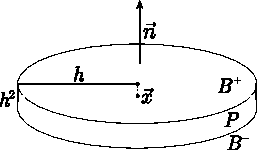
\includegraphics[width=0.6\textwidth]{images/sample.pdf}
%% \caption[caption za v kazalo]{Dolg caption pod sliko}
%  \caption[Primer vektorske slike.]{Primer vektorske slike z oznakami v enaki pisavi, kot jo
%     uporablja \LaTeX{}.  Narejena je s programom Inkscape, \LaTeX{} oznake so importane v
%     Inkscape iz pomožnega PDF.}
%  \label{fig:sample}
%\end{figure}
%
%\begin{figure}[h]
%  \centering
%  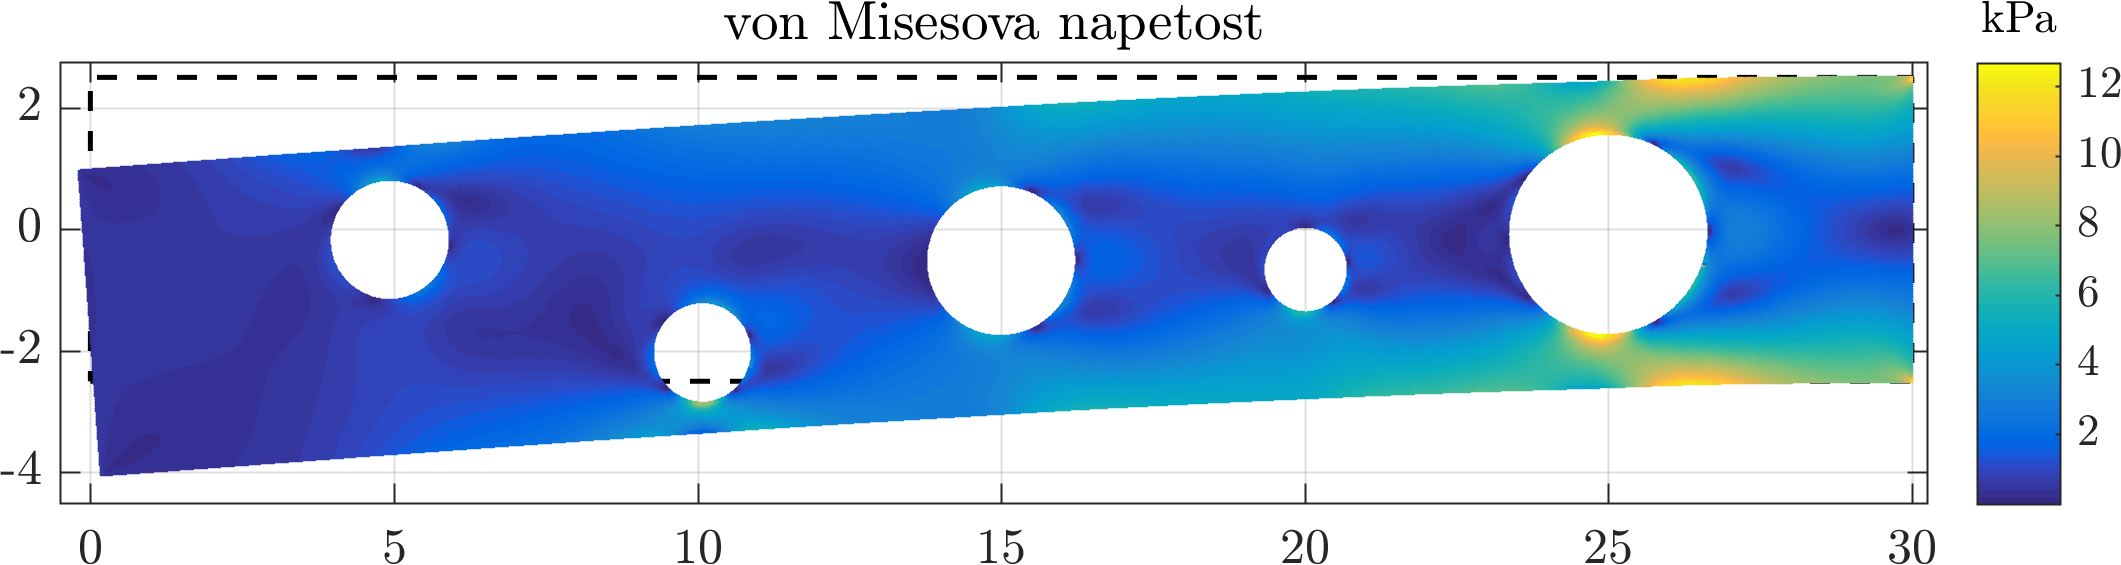
\includegraphics[width=0.8\textwidth]{images/image.png}
%  \caption[Primer bitne slike.]{Primer bitne slike, izvožene iz Matlaba. Poskrbite, da so slike v
%  dovolj visoki resoluciji in da ne vsebujejo prosojnih elementov (to zahteva PDF/A-1b format).}
%  \label{fig:image}
%\end{figure}
%
%\subsection{Kako narediti stvarno kazalo}
%Dodate ukaze \verb|\index{polje}| na besede, kjer je pojavijo, kot tukaj\index{tukaj}.
%Več o stvarnih kazalih je na voljo na \url{https://en.wikibooks.org/wiki/LaTeX/Indexing}.
%
%\subsection{Navajanje literature}
%%Članke citiramo z uporabo \verb|\cite{label}|, \verb|\cite[text]{label}| ali pa več naenkrat s
%%\verb|\cite\{label1, label2}|. Tudi tukaj predhodno besedo in citat povežemo z nedeljivim presledkom
%%$\sim$. Na primer~\cite{chen2006meshless,liu2001point}, ali pa \cite{kibriya2007empirical}, ali pa
%%\cite[str.\ 12]{trobec2015parallel}, \cite[enačba (2.3)]{pereira2016convergence}.
%%Vnosi iz \verb|.bib| datoteke, ki niso citirani, se ne prikažejo v seznamu literature, zato jih
%%tukaj citiram.~\cite{vene2000categorical}, \cite{gregoric2017stopniceni}, \cite{slak2015induktivni},
%%\cite{nsphere}, \cite{kearsley1975linearly}, \cite{STtemplate}, \cite{NunbergerTand}.
%
%Tu na novo citiram \cite{DPHclanek1}, \cite{DPHclanek2}, \cite{beltranmonterde}, \cite{choi2002clifford},
%\cite{struik1961lectures}, \cite{kreyszig2019differential}, \cite{faroukietal2004}, \cite{farouki2008pythagorean}. 

% Literatura:
% Primer navajanja na http://www.fmf.uni-lj.si/storage/24240/LiteraturaM.pdf,
% ampak bi moral stil poskrbeti za vse. Reference se uredijo po abecedi.
% Če nobena izbira izmed @book, @atricle,... ni ok, potem se lahko vse napiše v
% @misc pod note={} in deluje tako kot normalen LaTeX.
% Komentar v bib datoteki se naredi samo s parom { }
% Za urejanje literature avtor priporoča program Jabref, ki zna tudi avtomatsko
% okrajšati imena revij. Za pravilno sortiranje vnosov brez avtorja, uporabite
% polje key={ }, kot v primeru.
% V primeru napak ustvarite issue na GitHubu ali pišite na jure.slak@fmf.uni-lj.si.
\cleardoublepage                           % na desni strani
\phantomsection                            % da prav delujejo hiperlinki
\addcontentsline{toc}{section}{\bibname}   % dodajmo v kazalo
\bibliographystyle{fmf-sl}                 % uporabljen stil je v datoteki fmf-sl.bst, na voljo tudi angleška verzija
\bibliography{literatura.bib}                 % literatura je v datoteki, definirani na začetku
% TeXStudio zmede \ zgoraj, tako da lahko notri napišeš dejansko ime .bib datoteke, če ti
% ne delajo predlogi citatov.

% Za stvarno kazalo
\cleardoublepage                           % na desni strani
\phantomsection                            % da prav delujejo hiperlinki
\addcontentsline{toc}{section}{\indexname} % dodajmo v kazalo
\printindex

\end{document}
